\documentclass[12pt,a4paper]{report}

% ---------- Encodage, langue et typographie ----------
\usepackage[utf8]{inputenc}
\usepackage[T1]{fontenc}
\usepackage[french]{babel}
\usepackage{lmodern}
\renewcommand{\familydefault}{\sfdefault}
\usepackage{microtype}
\usepackage{tikz}
\usetikzlibrary{calc, shapes.geometric, decorations.pathreplacing, arrows.meta, positioning, fit, backgrounds}



% ---------- Mise en page ----------
\usepackage[a4paper,top=2.8cm,bottom=2.8cm,left=2.5cm,right=2.5cm]{geometry}
\usepackage{setspace}
\setstretch{1.3}
\usepackage{parskip}

% ---------- Couleurs ----------
\usepackage{xcolor}
\definecolor{primary}     {RGB}{15, 23, 42}
\definecolor{secondary}   {RGB}{51, 65, 85}
\definecolor{accent}      {RGB}{2, 132, 199}
\definecolor{accentlight} {RGB}{14, 165, 233}
\definecolor{lightgray}   {RGB}{241, 245, 249}
\definecolor{midgray}     {RGB}{203, 213, 225}
\definecolor{pagebg}      {HTML}{0A0F1E}
\definecolor{accentblue}  {HTML}{00B4FF}
\definecolor{accentteal}  {HTML}{00D4B4}
\definecolor{accentviolet}{HTML}{A78BFA}
\definecolor{accentamber} {HTML}{F59E0B}
\definecolor{textprimary} {HTML}{FFFFFF}
\definecolor{textsec}     {HTML}{8899AA}
\definecolor{borderfaint} {HTML}{1E2A3A}
\definecolor{cardbg}      {HTML}{111827}
\definecolor{cardline}    {HTML}{2A3A4A}
\definecolor{bronzeC}     {HTML}{C97A55}
\definecolor{silverC}     {HTML}{8A95A3}
\definecolor{goldC}       {HTML}{D4A848}
\definecolor{postgresC}   {HTML}{336791}

\usepackage{graphicx}
\usepackage{float}
\usepackage{array}
\usepackage{tabularx}
\usepackage{booktabs}
\usepackage{longtable}
\usepackage{colortbl}
\renewcommand{\arraystretch}{1.4}

% ---------- Titres ----------
\usepackage{titlesec}
\titleformat{\chapter}[display]
  {\normalfont\bfseries\color{primary}}
  {\begin{tikzpicture}
    \node[fill=accent, text=white, rounded corners=3pt,
          inner xsep=10pt, inner ysep=8pt, font=\Large\bfseries]
      {\chaptertitlename\ \thechapter};
  \end{tikzpicture}}
  {1ex}{\Huge\titlerule[0pt]\vspace{1ex}}
\titlespacing*{\chapter}{0pt}{-20pt}{25pt}

\titleformat{\section}[hang]
  {\normalfont\LARGE\bfseries\color{primary}}
  {\color{accent}\thesection.}{0.8em}{}
  [\vspace{-0.5ex}{\color{midgray}\titlerule[1pt]}]

\titleformat{\subsection}[hang]
  {\normalfont\Large\bfseries\color{secondary}}
  {\color{accentlight}\thesubsection}{0.8em}{}

% ---------- En-têtes / pieds ----------
\usepackage{fancyhdr}
\pagestyle{fancy}
\fancyhf{}
\renewcommand{\headrulewidth}{0.5pt}
\renewcommand{\headrule}{%
  \hbox to\headwidth{\color{midgray}\leaders\hrule height \headrulewidth\hfill}}
\renewcommand{\footrulewidth}{0pt}
\fancyhead[L]{\small\color{secondary}\textbf{Data Breach \& Threat Intelligence Monitoring Platform}}


\fancyfoot[C]{%
  \begin{tikzpicture}
    \node[fill=lightgray, text=primary, rounded corners=2pt,
          inner xsep=6pt, inner ysep=3pt, font=\small\bfseries] {\thepage};
  \end{tikzpicture}}

% ---------- Hyperliens ----------
\usepackage[hidelinks]{hyperref}
\hypersetup{
  colorlinks=true, linkcolor=primary,
  filecolor=accent, urlcolor=accent, citecolor=secondary,
  pdftitle={Data Breach \& Threat Intelligence Monitoring Platform},
  pdfauthor={Équipe projet Data Breach \& Threat Intelligence Monitoring Platform}
}

% ---------- Listes ----------
\usepackage{enumitem}
\setlist{itemsep=4pt,topsep=6pt}

\setlist[itemize]{
  itemsep=0pt,
  parsep=0pt,
  topsep=2pt,
  partopsep=0pt,
  leftmargin=*
}

% ---------- Encadrés ----------
\usepackage{tcolorbox}
\tcbuselibrary{skins,breakable}

\newtcolorbox{infoBox}[1][]{
  enhanced, breakable,
  colback=lightgray, colframe=primary, boxrule=1.5pt,
  fonttitle=\bfseries\large, coltitle=white,
  attach boxed title to top left={xshift=5mm,yshift=-3.5mm},
  boxed title style={colback=primary, rounded corners=2pt, boxrule=0pt},
  rounded corners, arc=3mm,
  left=5mm, right=5mm, top=5mm, bottom=5mm,
  drop shadow=black!10!white, #1
}

\newcommand{\projetnom}{Data Breach \& Threat Intelligence Monitoring Platform}
\newcommand{\platformename}{plateforme de veille \projetnom{}}

\newcommand{\screenshotplaceholder}[2]{%
  \begin{figure}[H]
    \centering
    \begin{tcolorbox}[
      enhanced, colback=lightgray, colframe=midgray,
      boxrule=1.5pt, arc=3mm, width=0.9\linewidth,
      drop shadow=black!5!white, halign=center, valign=center, height=6.5cm
    ]
      \vspace{0.8cm}
      \begin{tikzpicture}
        \node[fill=midgray!50, text=secondary, rounded corners=3pt,
              inner xsep=8pt, inner ysep=5pt, font=\bfseries]
          {Emplacement réservé pour capture d'écran};
      \end{tikzpicture}\\[12pt]
      \textcolor{primary}{\large\textbf{#1}}\\[8pt]
      {\small\color{secondary}\itshape
        (Remplacer par :
        \texttt{\textbackslash includegraphics[width=0.9\textbackslash linewidth]\{#2\}})}
    \end{tcolorbox}
    \caption{#1}
    \label{fig:#2}
  \end{figure}
}

% =============================================================================
%  LAYOUT CONSTANTS
%  A4 = 210mm. Content zone 80% = 168mm centred → left edge = 2.1cm
%  W=16.8cm  L=2.1cm  R=18.9cm
%  Twin cards: each 8.2cm, gutter 0.4cm, right card at x=10.7cm
% =============================================================================

\begin{document}

% =============================================================================
%  PAGE DE GARDE — STYLE EXECUTIVE CYBER INTELLIGENCE (FIXED)
% =============================================================================
\begin{titlepage}
\thispagestyle{empty}

\begin{tikzpicture}[remember picture, overlay]

  % -----------------------------------------------------------------------
  % 1. BACKGROUND & GEOMETRIC SHAPES
  % -----------------------------------------------------------------------
  \fill[white] (current page.south west) rectangle (current page.north east);

  % Bandeau supérieur élégant (Primary + Accent)
  \fill[primary] 
    (current page.north west) -- 
    (current page.north east) -- 
    ([yshift=-4.5cm]current page.north east) .. controls 
    ([yshift=-4.5cm, xshift=-5cm]current page.north) and 
    ([yshift=-7cm, xshift=3cm]current page.north west) .. 
    ([yshift=-8cm]current page.north west) -- cycle;
    
  \fill[accent, opacity=0.8] 
    ([yshift=-8cm]current page.north west) .. controls 
    ([yshift=-7cm, xshift=3cm]current page.north west) and 
    ([yshift=-4.5cm, xshift=-5cm]current page.north) .. 
    ([yshift=-4.5cm]current page.north east) -- 
    ([yshift=-4.8cm]current page.north east) .. controls 
    ([yshift=-4.8cm, xshift=-5cm]current page.north) and 
    ([yshift=-7.3cm, xshift=3cm]current page.north west) .. 
    ([yshift=-8.3cm]current page.north west) -- cycle;

  % -----------------------------------------------------------------------
  % 1.B GEOMETRIC CORNER DECORATION (Bottom Right — replaces the diagram)
  % -----------------------------------------------------------------------
  % Subtle triangular corner fill
  \fill[lightgray] 
    (current page.south east) -- 
    ([yshift=4cm]current page.south east) -- 
    ([xshift=-4cm]current page.south east) -- cycle;
    
  \fill[accent!10] 
    ([xshift=-4cm]current page.south east) -- 
    ([yshift=4cm]current page.south east) -- 
    ([xshift=-1.2cm, yshift=5.5cm]current page.south east) -- 
    ([xshift=-5.5cm, yshift=1.2cm]current page.south east) -- cycle;

  \draw[accent, line width=2pt, opacity=0.3] 
    ([xshift=-5cm, yshift=0cm]current page.south east) -- 
    ([xshift=0cm, yshift=5cm]current page.south east);



  % -----------------------------------------------------------------------
  % 2. LOGO & EN-TÊTE
  % -----------------------------------------------------------------------
  \node[anchor=north east, xshift=-2cm, yshift=-1.5cm] 
    at (current page.north east) {
 {
        
\includegraphics[width=10cm, height=3cm, keepaspectratio]{images/logo.png}
      };
    };

  \node[anchor=north west, xshift=2.5cm, yshift=-2.5cm] 
    at (current page.north west) {
      {\sffamily\fontsize{16}{16}\selectfont\bfseries\color{accentlight}
      RAPPORT DE PROJET}
    };

  \node[anchor=north west, xshift=2.5cm, yshift=-3.2cm] 
    at (current page.north west) {
      {\sffamily\fontsize{12}{12}\selectfont\color{white!80}
      Année universitaire 2025 -- 2026}
    };

  % -----------------------------------------------------------------------
  % 3. TITRE PRINCIPAL
  % -----------------------------------------------------------------------
  \node[anchor=north west, xshift=2.5cm, yshift=-10cm] 
    at (current page.north west) {
      \begin{minipage}{14cm}  % ← narrowed to leave right margin clear
        {\sffamily\fontsize{42}{48}\selectfont\bfseries\color{primary}
        Data Breach}\\[6pt]
        {\sffamily\fontsize{34}{40}\selectfont\bfseries\color{secondary}
        \& Threat Intelligence}\\[8pt]
        {\sffamily\fontsize{26}{32}\selectfont\bfseries\color{accent}
        Monitoring Platform}
      \end{minipage}
    };

  % Séparateur
  \draw[accent, line width=3pt, line cap=round] 
    ([xshift=2.6cm,yshift=-15.2cm]current page.north west) -- 
    ([xshift=6cm,yshift=-15.2cm]current page.north west);

  % Sous-titre
  \node[anchor=north west, xshift=2.5cm, yshift=-16cm] 
    at (current page.north west) {
      \begin{minipage}{13cm}  % ← narrowed so text stays left of diagram
        {\sffamily\fontsize{14}{18}\selectfont\color{secondary}
        \textbf{Plateforme de veille cyber multi-sources} dédiée à la détection, 
        la qualification et la visualisation des expositions publiques, 
        des signaux OSINT communautaires et des vulnérabilités CVE.}
      \end{minipage}
    };

  % Mots-clés (Badges modernes)
  \node[anchor=north west, xshift=2.5cm, yshift=-18.5cm] 
    at (current page.north west) {
      \begin{tikzpicture}
        \tikzstyle{badge} = [
          fill=accent!10, text=primary,
          font=\sffamily\footnotesize\bfseries,
          rounded corners=4pt, inner xsep=10pt, inner ysep=6pt
        ]
        \node[badge] (b1) {OSINT};
        \node[badge, right=8pt of b1] (b2) {DATA BREACH};
        \node[badge, right=8pt of b2] (b3) {THREAT INTELLIGENCE};
        \node[badge, right=8pt of b3] (b4) {BUSINESS INTELLIGENCE};
      \end{tikzpicture}
    };

  % -----------------------------------------------------------------------
  % 4. AUTEURS ET ENCADREMENT
  % -----------------------------------------------------------------------
  \draw[primary!20, line width=2pt] 
    ([xshift=2.6cm,yshift=-21cm]current page.north west) -- 
    ([xshift=2.6cm,yshift=-26cm]current page.north west);

  % Équipe projet
  \node[anchor=north west, xshift=3cm, yshift=-20.8cm] 
    at (current page.north west) {
      \begin{minipage}{6.5cm}
        {\sffamily\fontsize{10}{12}\selectfont\bfseries\color{accent}
        RÉALISÉ PAR}\\[6pt]
        {\sffamily\fontsize{12}{15}\selectfont\bfseries\color{primary}
        Hamza Bjibji}\\[2pt]
        {\sffamily\fontsize{12}{15}\selectfont\bfseries\color{primary}
        Chaimae Ben Sbeh}\\[2pt]
        {\sffamily\fontsize{12}{15}\selectfont\bfseries\color{primary}
        Imane Sghiouar}\\[2pt]
        {\sffamily\fontsize{12}{15}\selectfont\bfseries\color{primary}
        Yassir Salim El Akramine}
      \end{minipage}
    };

  % Encadrant
  \node[anchor=north west, xshift=10.5cm, yshift=-20.8cm] 
    at (current page.north west) {
      \begin{minipage}{7cm}
        {\sffamily\fontsize{10}{12}\selectfont\bfseries\color{accent}
        ENCADRÉ PAR}\\[6pt]
        {\sffamily\fontsize{12}{15}\selectfont\bfseries\color{primary}
        Prof. Younes Wadiai}
      \end{minipage}
    };

  % Filière
  \node[anchor=north west, xshift=10.5cm, yshift=-23.5cm] 
    at (current page.north west) {
      \begin{minipage}{7cm}
        {\sffamily\fontsize{10}{12}\selectfont\bfseries\color{accent}
        FILIÈRE}\\[6pt]
        {\sffamily\fontsize{12}{15}\selectfont\bfseries\color{primary}
        Big Data \& Intelligence Artificielle}
      \end{minipage}
    };

  % -----------------------------------------------------------------------
  % 5. PIED DE PAGE
  % -----------------------------------------------------------------------
  \node[anchor=south west, xshift=2.5cm, yshift=1.5cm] 
    at (current page.south west) {
      {\sffamily\fontsize{10}{12}\selectfont\color{secondary}
      Rapport de projet -- \today}
    };

\end{tikzpicture}
\end{titlepage}





% =============================================================================
%  RÉSUMÉ
% =============================================================================
\chapter*{Résumé}
\addcontentsline{toc}{chapter}{Résumé}

Le projet \textit{\projetnom{}} propose une \platformename{} dédiée à la détection des expositions publiques de données sensibles. La plateforme agrège et corrèle plusieurs sources ouvertes : \textbf{GitHub} pour les fuites techniques de secrets, \textbf{Telegram} pour la veille communautaire et CVE, \textbf{Google Alerts} pour la dimension OSINT et médiatique, ainsi qu'un module complémentaire de \textit{Threat Intelligence} consacré aux flux CVE et à la production de tableaux de bord BI.

L'approche retenue est méthodologique : chaque source est configurée à partir de fichiers de référence, les données collectées sont normalisées, analysées, puis filtrées par une \textit{detection policy} avant d'être classifiées par catégorie de risque et par niveau de criticité. Les signaux qualifiés sont ensuite stockés, visualisés dans des tableaux de bord interactifs et exploités par l'analyste pour la prise de décision.


% =============================================================================
%  TABLE DES MATIÈRES
% =============================================================================
\tableofcontents
\thispagestyle{fancy}


% =============================================================================
%  CHAPITRE 1 — CONTEXTE, OBJECTIFS ET PÉRIMÈTRE DU PROJET
% =============================================================================
\chapter{Contexte, objectifs et périmètre du projet}

\section{Contexte général}

Le projet \textit{\projetnom{}} a été conçu pour répondre à un constat simple : une grande quantité d'informations sensibles apparaît quotidiennement sur des espaces publics. Il peut s'agir de secrets techniques, d'identifiants, de mentions de fuites de données, de vulnérabilités publiées ou encore de signaux communautaires liés à des incidents cyber.

Ces expositions sont rarement intentionnelles, mais elles représentent un risque de sécurité important. Un secret oublié dans un dépôt public, une annonce de fuite sur un canal OSINT ou une vulnérabilité critique récemment publiée peuvent constituer des éléments exploitables par un attaquant.

Dans ce contexte, le projet vise à fournir une plateforme de veille défensive capable de centraliser, qualifier et restituer ces signaux à un analyste.

\section{Objectif global}

L'objectif principal de la plateforme est de collecter, normaliser, filtrer et présenter des signaux cyber issus de sources ouvertes et autorisées. La solution permet de gagner du temps sur la collecte manuelle, de réduire la dispersion de l'information et de fournir un cadre cohérent pour prioriser les détections.

Le projet ne vise pas à mener des actions offensives. Il s'inscrit dans une logique de \textbf{veille défensive}, d'\textbf{OSINT} et de \textbf{Threat Intelligence}. Son rôle est d'aider l'analyste à identifier rapidement les signaux pertinents, à comprendre leur criticité et à suivre leur évolution.

\section{Périmètre fonctionnel}

Du point de vue fonctionnel, la plateforme assure trois grands rôles.

\begin{itemize}
  \item \textbf{Collecte multi-sources} : interrogation de GitHub pour les fuites techniques, Telegram pour les signaux communautaires, Google Alerts pour la veille médiatique et les flux CVE pour l'analyse des vulnérabilités.
  \item \textbf{Traitement et qualification} : analyse de contenu, application d'une \textit{detection policy}, déduplication, redaction et classification selon le niveau de risque.
  \item \textbf{Restitution analytique} : visualisation des signaux dans des tableaux de bord permettant à l'analyste de suivre l'état des sources, les résultats collectés et les tendances observées.
\end{itemize}

\section{Public cible}

Ce périmètre s'adresse principalement à :

\begin{itemize}
  \item un \textbf{analyste SOC} chargé de la veille quotidienne ;
  \item un \textbf{responsable sécurité} souhaitant suivre des indicateurs de risque ;
  \item un \textbf{enseignant ou chercheur} voulant illustrer une chaîne de veille OSINT complète ;
  \item une équipe projet souhaitant expérimenter une architecture de collecte, de traitement et de visualisation cyber.
\end{itemize}

\section{Vision méthodologique}

Ce projet traite la veille cyber comme un processus méthodologique et non comme une simple accumulation de résultats. La plateforme repose sur quatre principes directeurs :

\begin{itemize}
  \item \textbf{séparation des responsabilités} : chaque source dispose de son propre collecteur ;
  \item \textbf{configuration externalisée} : les requêtes, canaux et alertes sont décrits dans des fichiers dédiés ;
  \item \textbf{filtrage explicite} : les règles de validation, de scoring et de redaction sont centralisées ;
  \item \textbf{approche défensive} : les données sensibles ne sont pas conservées en clair.
\end{itemize}

Cette vision permet de construire une plateforme plus lisible, plus maintenable et plus facilement auditable.

% =============================================================================
%  CHAPITRE 2 — ARCHITECTURE GÉNÉRALE ET MÉTHODOLOGIE DE VEILLE
% =============================================================================
\chapter{Architecture générale et méthodologie de veille}

\section{Vue d'ensemble de l'architecture}

La plateforme repose sur une architecture modulaire organisée autour d'un pipeline de veille. Ce pipeline couvre les étapes principales suivantes : configuration des sources, collecte, normalisation, analyse, filtrage, redaction, stockage et restitution à l'analyste.

La figure~\ref{fig:pipeline-diagram} synthétise l'écosystème complet du projet en distinguant deux sous-systèmes complémentaires. Le premier correspond à la plateforme principale de monitoring, orientée vers la détection d'expositions publiques. Le second correspond au module \textit{BI Threat Intelligence}, orienté vers l'exploitation analytique des flux CVE.

\begin{figure}[H]
    \centering
    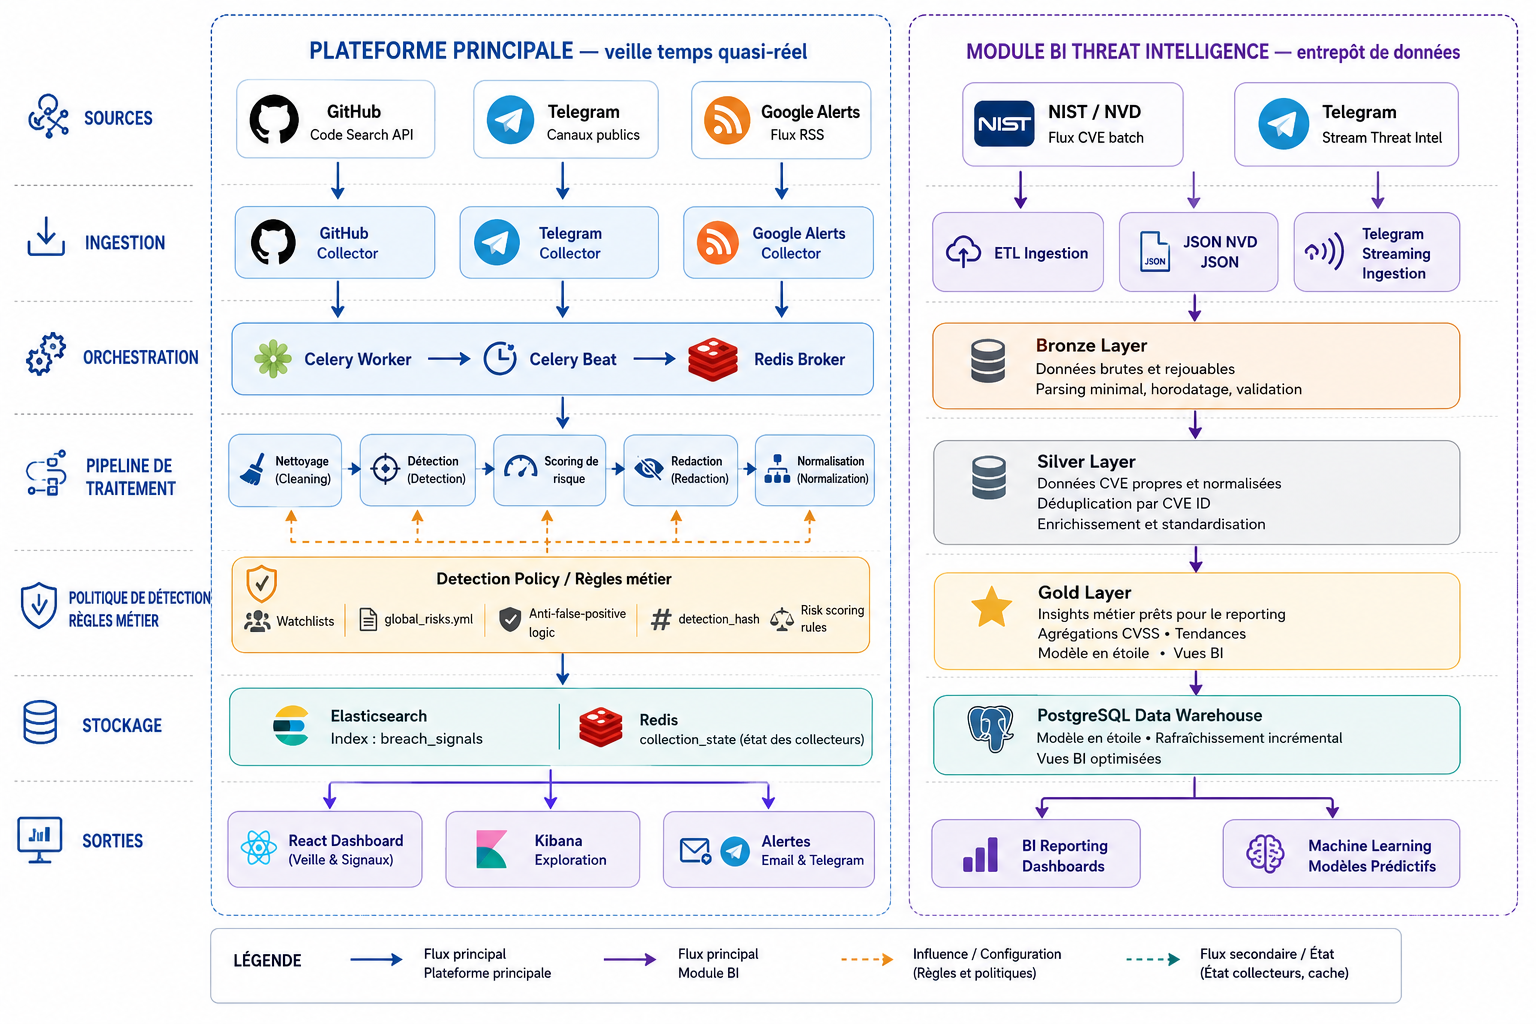
\includegraphics[width=.95\linewidth]{images/diagramme_concep.png}
    \caption{Vue conceptuelle du pipeline global de veille}
    \label{fig:pipeline-diagram}
\end{figure}

\section{Plateforme principale de monitoring}
La plateforme principale collecte des signaux depuis plusieurs sources OSINT, notamment GitHub, Telegram et Google Alerts. Chaque source dispose de son propre collecteur afin de séparer les responsabilités et de faciliter l'évolution du système. Après la collecte, les résultats passent par une chaîne d'analyse qui extrait les informations utiles, normalise les données, applique la \textit{detection policy}, calcule un score de risque, attribue une sévérité et un niveau de confiance, puis redacte les données sensibles avant de stocker uniquement les signaux qualifiés.

\section{Module BI Threat Intelligence}

Le module \textit{BI Threat Intelligence} constitue un sous-projet complémentaire. Son objectif n'est pas de détecter directement des secrets exposés, mais d'exploiter les flux \textbf{Common Vulnerabilities and Exposures} afin de produire des indicateurs décisionnels.

Ce module repose sur une architecture de type \textbf{Data Warehouse} organisée selon le modèle médaillon : Bronze, Silver et Gold. Les données CVE sont d'abord collectées à l'état brut, puis nettoyées et enrichies avant d'être transformées en tables exploitables par Power BI.

\section{Configuration des sources}

La plateforme utilise des fichiers de configuration externes pour définir les sources, les requêtes, les alertes et les règles de détection. Cette approche évite de modifier le code à chaque changement et rend la veille plus claire, maintenable et auditable.



\begin{table}[H]
\centering
\caption{Fichiers de configuration utilisés par la plateforme}
\label{tab:config-files}
\begin{tabularx}{\linewidth}{|l|>{\raggedright\arraybackslash}X|}
\hline
\rowcolor{primary!15}
\textbf{Fichier} & \textbf{Rôle} \\ \hline
Fichier des risques globaux GitHub & Catégories de risques et requêtes de recherche utilisées pour détecter les expositions techniques \\ \hline
Fichier des canaux Telegram & Liste des canaux publics suivis, catégories associées et paramètres de collecte. \\ \hline
Fichier des alertes Google Alerts & Alertes RSS catégorisées permettant d'assurer la veille médiatique et OSINT. \\ \hline
Fichier de \textit{detection policy} & Règles de filtrage, motifs placeholders, scoring, classification et traitement des faux positifs. \\ \hline
\end{tabularx}
\end{table}



\section{Contrôle des sources}

Chaque source dispose d'un état observable dans la plateforme. Cet état permet à l'analyste de vérifier si une source fonctionne correctement ou si elle présente des erreurs.

\begin{itemize}
  \item état technique : \textit{healthy}, \textit{warning}, \textit{error}, \textit{disabled} ;
  \item dernier passage de collecte et résultat associé ;
  \item nombre d'éléments collectés, dédupliqués et indexés ;
  \item compteurs d'erreurs et d'avertissements.
\end{itemize}

Ce contrôle continu permet d'expliquer pourquoi une source ne produit pas de nouvelles détections, par exemple lorsque les éléments collectés sont déjà connus ou filtrés par la politique de détection.


\begin{figure}[H]
    \centering
    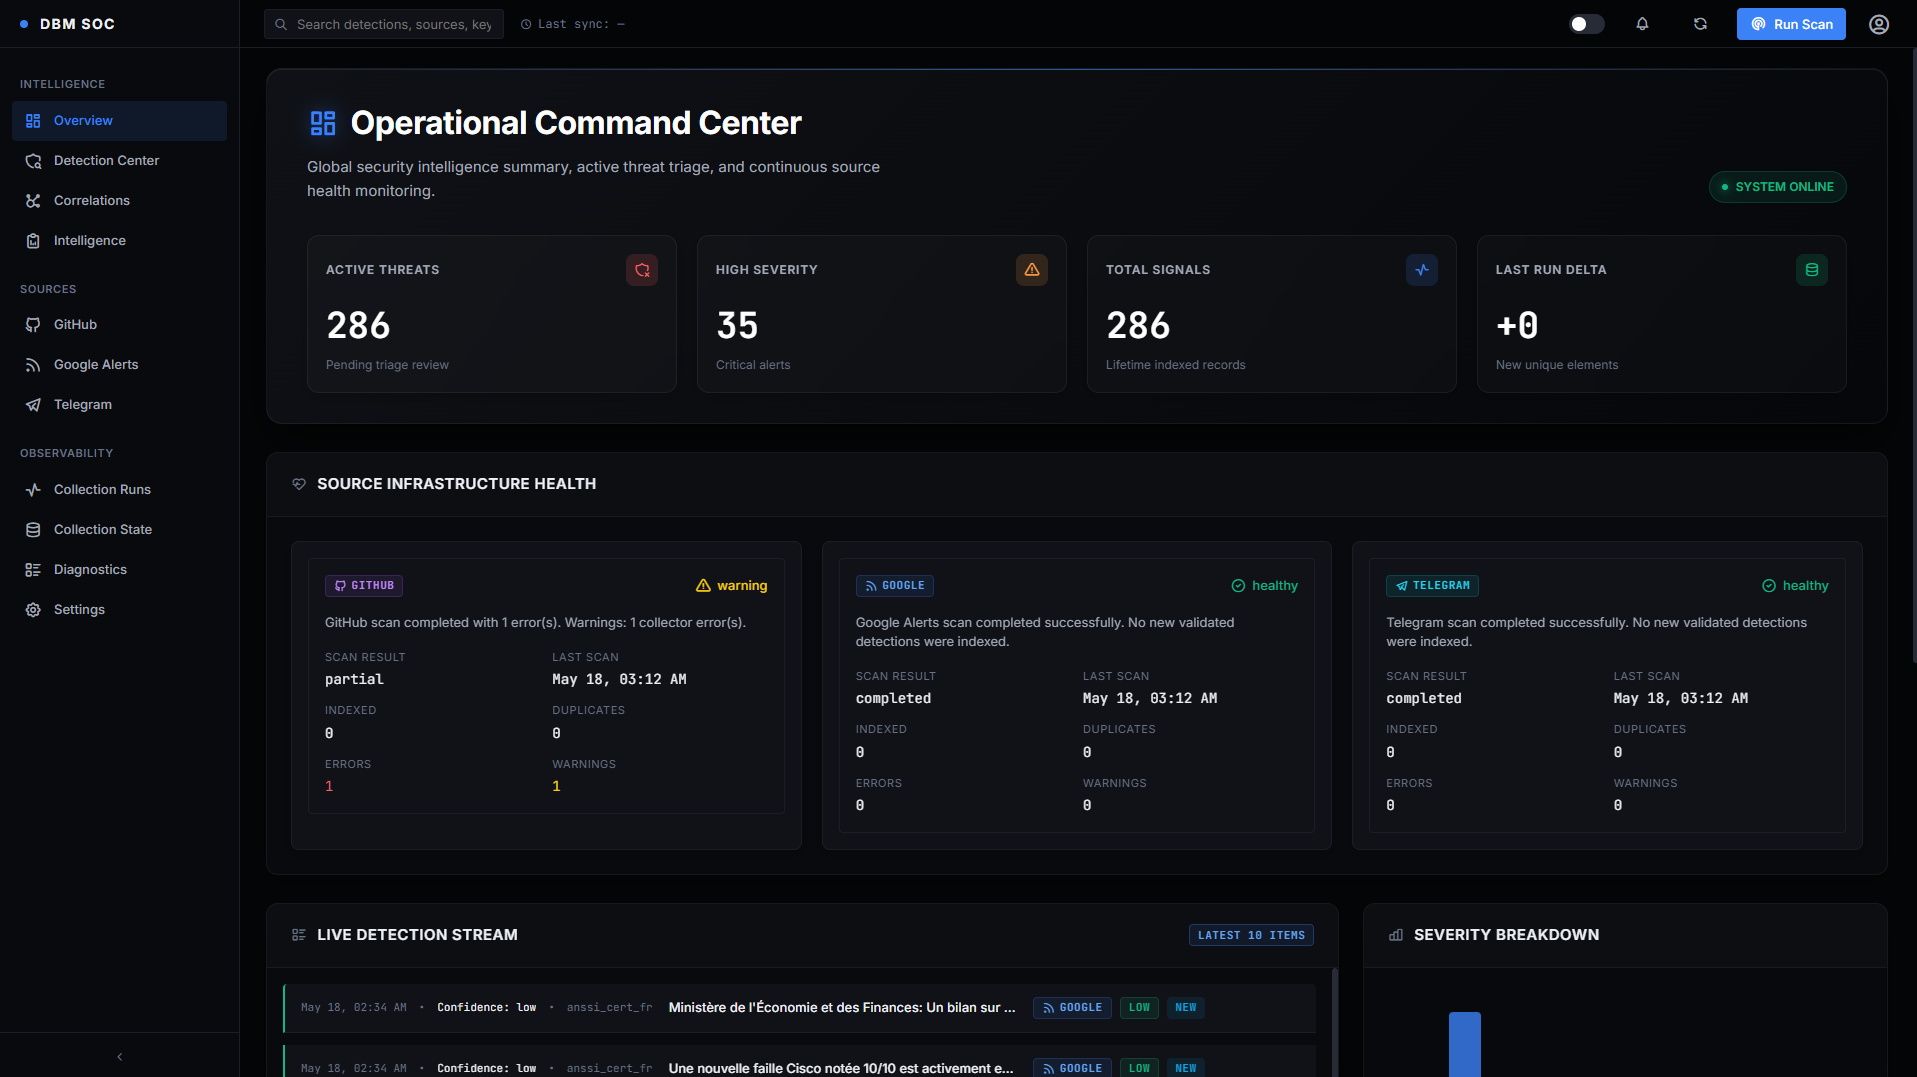
\includegraphics[width=1\linewidth]{images/overview.png}
\end{figure}



% =============================================================================
%  CHAPITRE 3 — SOURCES DE DONNÉES ET STRATÉGIE DE COLLECTE
% =============================================================================
\chapter{Sources de données et stratégie de collecte}

\section{Vue d'ensemble des sources}

La plateforme s'appuie sur quatre familles de sources complémentaires. Chacune apporte un type de signal différent : technique, communautaire, médiatique ou vulnérabilité.

\begin{table}[H]
\centering
\caption{Vue d'ensemble des sources intégrées dans la plateforme}
\label{tab:sources-overview}
\begin{tabularx}{\linewidth}{|l|>{\raggedright\arraybackslash}X|>{\raggedright\arraybackslash}X|}
\hline
\rowcolor{primary!15}
\textbf{Source} & \textbf{Type de signal} & \textbf{Apport principal} \\ \hline
GitHub & Fuites techniques de secrets & Preuves d'exposition directe \\ \hline
Telegram & Canaux publics OSINT / CVE & Signaux communautaires précoces \\ \hline
Google Alerts & Veille médiatique RSS & Couverture news et OSINT \\ \hline
CVE Feed / BI Threat Intelligence & Vulnérabilités publiées & Vision quantitative et tendancielle \\ \hline
\end{tabularx}
\end{table}

\newpage
\section{GitHub Monitoring}

\subsection{Rôle de la source}

GitHub représente l'une des sources principales de collecte de notre plateforme, car il permet d'identifier des preuves techniques d'exposition directement présentes dans des dépôts publics. De nombreux projets publiés sur GitHub peuvent contenir, volontairement ou par erreur, des secrets applicatifs tels que des fichiers \texttt{.env}, des clés d'API, des tokens d'accès, des certificats, des identifiants de bases de données ou encore des chaînes de connexion.

\subsection{Mécanisme d'accès}

L'accès aux données GitHub est réalisé à travers l'API officielle \textbf{GitHub Code Search}. Un \textit{token développeur GitHub} est utilisé afin d'authentifier les requêtes et de bénéficier de quotas plus adaptés aux opérations de recherche automatisée.

Le module exécute des requêtes ciblées sur le code public, collecte les résultats candidats, puis analyse le contenu réel des fichiers afin de vérifier si l'exposition détectée correspond réellement à un secret exploitable ou à un simple faux positif.

\subsection{Organisation des requêtes}

La logique de recherche GitHub repose sur un fichier de configuration appelé \textbf{global risks}. Ce fichier centralise les requêtes de détection organisées par catégories de risques.

\begin{itemize}
  \item fichiers d'environnement : \texttt{.env}, \texttt{DATABASE\_URL}, \texttt{API\_KEY} ;
  \item identifiants de bases de données : PostgreSQL, MySQL, MongoDB, Supabase, Render ;
  \item clés d'API et tokens applicatifs ;
  \item secrets cloud : AWS, Azure, GCP ;
  \item secrets JWT et clés privées ;
  \item fichiers Docker, Kubernetes et fichiers de configuration applicative.
\end{itemize}

Chaque entrée contient une requête de recherche, une catégorie de risque et un niveau de sévérité indicatif. Cette organisation rend la veille plus structurée, auditable et évolutive.

\begin{figure}[H]
    \centering
    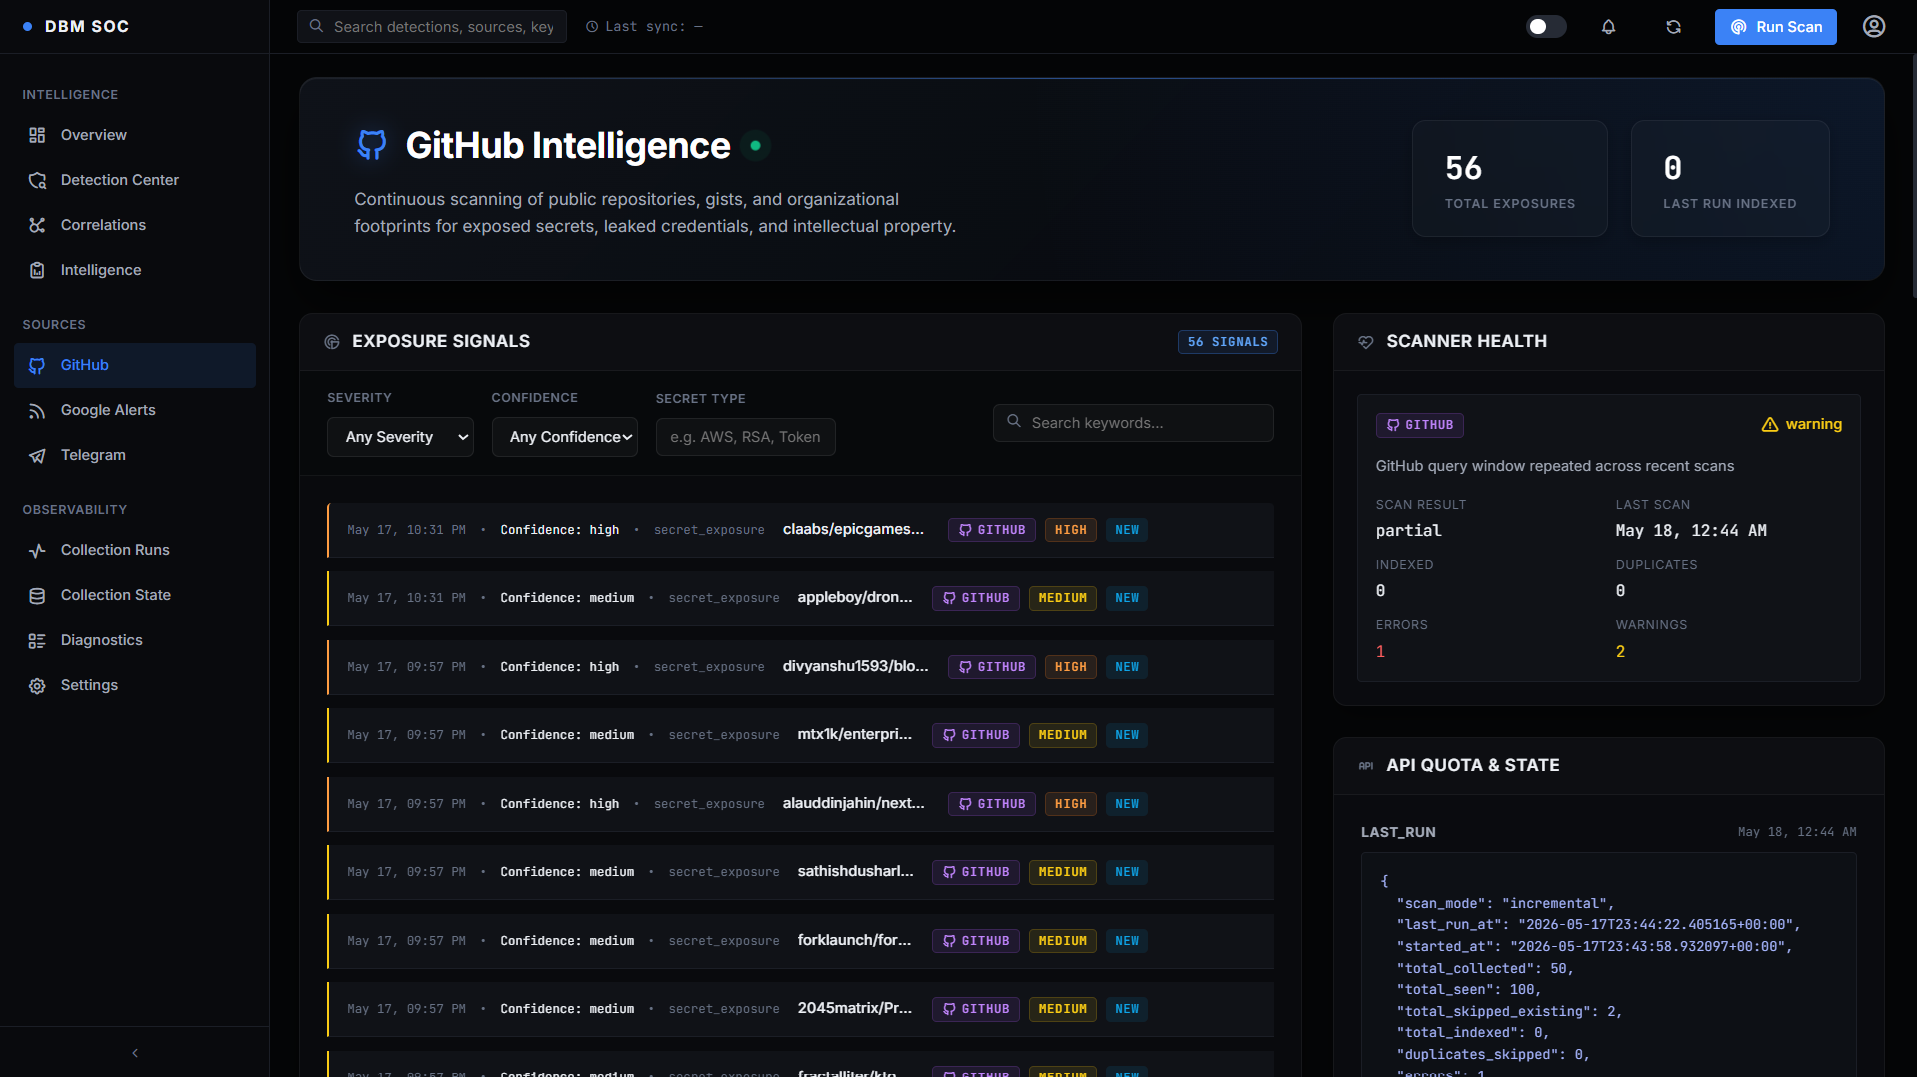
\includegraphics[width=.9\linewidth]{images/github_1.png}
    \caption{Interface GitHub Intelligence affichant les expositions collectées depuis GitHub}
    \label{fig:github-intelligence}
\end{figure}

La page \textbf{GitHub Intelligence} présente les résultats collectés depuis GitHub afin de détecter les secrets, credentials et expositions publiques. Le tableau central liste les signaux détectés avec leur sévérité, leur niveau de confiance, leur type de secret et leur statut. Les panneaux latéraux affichent l'état du scanner, le dernier scan, les erreurs, les avertissements et les données indexées.

\subsection{Exemple de résultat GitHub}

Parmi les résultats collectés, le système a identifié un cas d'exposition critique contenant plusieurs informations sensibles dans un fichier de configuration applicatif. Le contenu détecté incluait notamment :

\begin{itemize}
  \item des identifiants SMTP/Gmail utilisés pour l'envoi d'emails ;
  \item des URLs de bases de données PostgreSQL, Supabase et Render contenant des utilisateurs et mots de passe ;
  \item un secret Google OAuth ;
  \item des variables de connexion à une base de données : \texttt{HOST}, \texttt{PORT}, \texttt{USER}, \texttt{PASSWORD}.
\end{itemize}

Ce type de fuite est classé comme \textbf{secret exposure} avec une sévérité \textbf{high}, car il peut permettre à un attaquant d'accéder à des services backend, d'exploiter une base de données ou d'abuser de services tiers liés à l'application.

\begin{figure}[H]
    \centering
    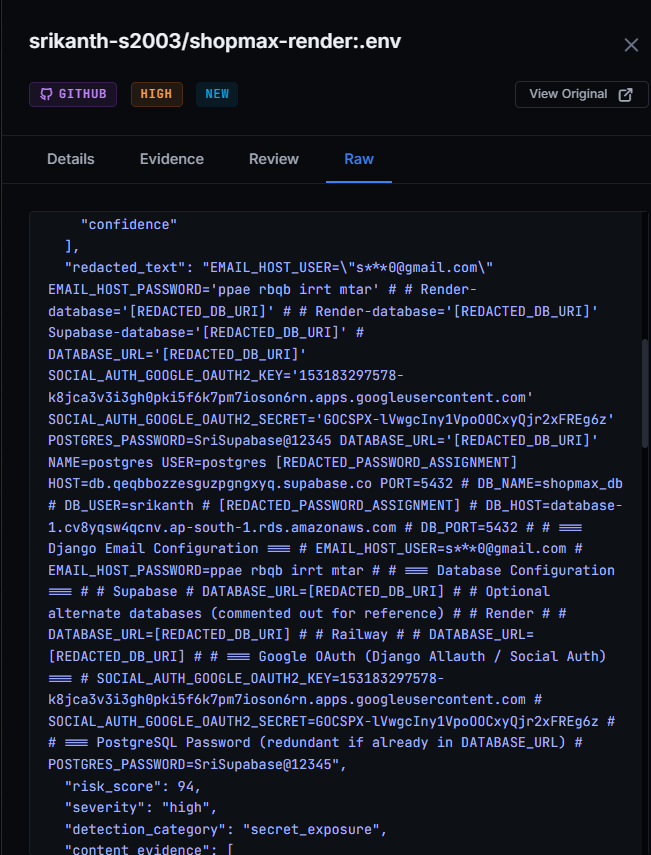
\includegraphics[width=.8\linewidth]{images/githubexposure.png}
    \caption{Exemple d'exposition critique détectée dans un dépôt GitHub public}
    \label{fig:github-exposure}
\end{figure}

\newpage
\section{Telegram Monitoring}

\subsection{Rôle de la source}

Telegram est utilisé comme une source de veille communautaire et OSINT. Certains canaux publics publient régulièrement des annonces liées aux fuites de données, aux vulnérabilités CVE, aux incidents cyber ou aux expositions revendiquées.

Contrairement à GitHub, qui fournit des preuves techniques directes à travers le code exposé, Telegram fournit principalement des indications déclaratives. Les informations collectées doivent donc être considérées comme des signaux à analyser et à valider, et non comme des preuves définitives.

\subsection{Canaux suivis}

La plateforme surveille actuellement deux canaux Telegram publics déclarés dans un fichier de configuration dédié.

\begin{table}[H]
\centering
\small
\caption{Canaux Telegram publics surveillés}
\label{tab:telegram-channels}
\renewcommand{\arraystretch}{1.05}
\begin{tabularx}{\linewidth}{|l|l|>{\raggedright\arraybackslash}X|}
\hline
\rowcolor{primary!15}
\textbf{Canal} & \textbf{Catégorie} & \textbf{Rôle} \\ \hline
CVEDetector & cve\_intelligence & Veille sur les CVE, vulnérabilités et alertes techniques. \\ \hline
breachforums\_cdn & data\_breaches & Suivi des annonces publiques liées aux fuites de données et aux expositions revendiquées. \\ \hline
\end{tabularx}
\end{table}

\subsection{Logique de traitement}

Les messages collectés depuis Telegram sont analysés, normalisés et transformés en signaux exploitables par le système.

\begin{itemize}
  \item extraction des informations utiles : titre, source, date, URLs, mots-clés et identifiants CVE ;
  \item détection des thématiques : fuite de données, vulnérabilité, exposition, compromission ou alerte technique ;
  \item classification du message selon sa catégorie ;
  \item génération d'un signal normalisé compatible avec le reste de la plateforme ;
  \item masquage ou réduction du contenu afin d'éviter le stockage inutile de données sensibles.
\end{itemize}

\begin{figure}[H]
    \centering
    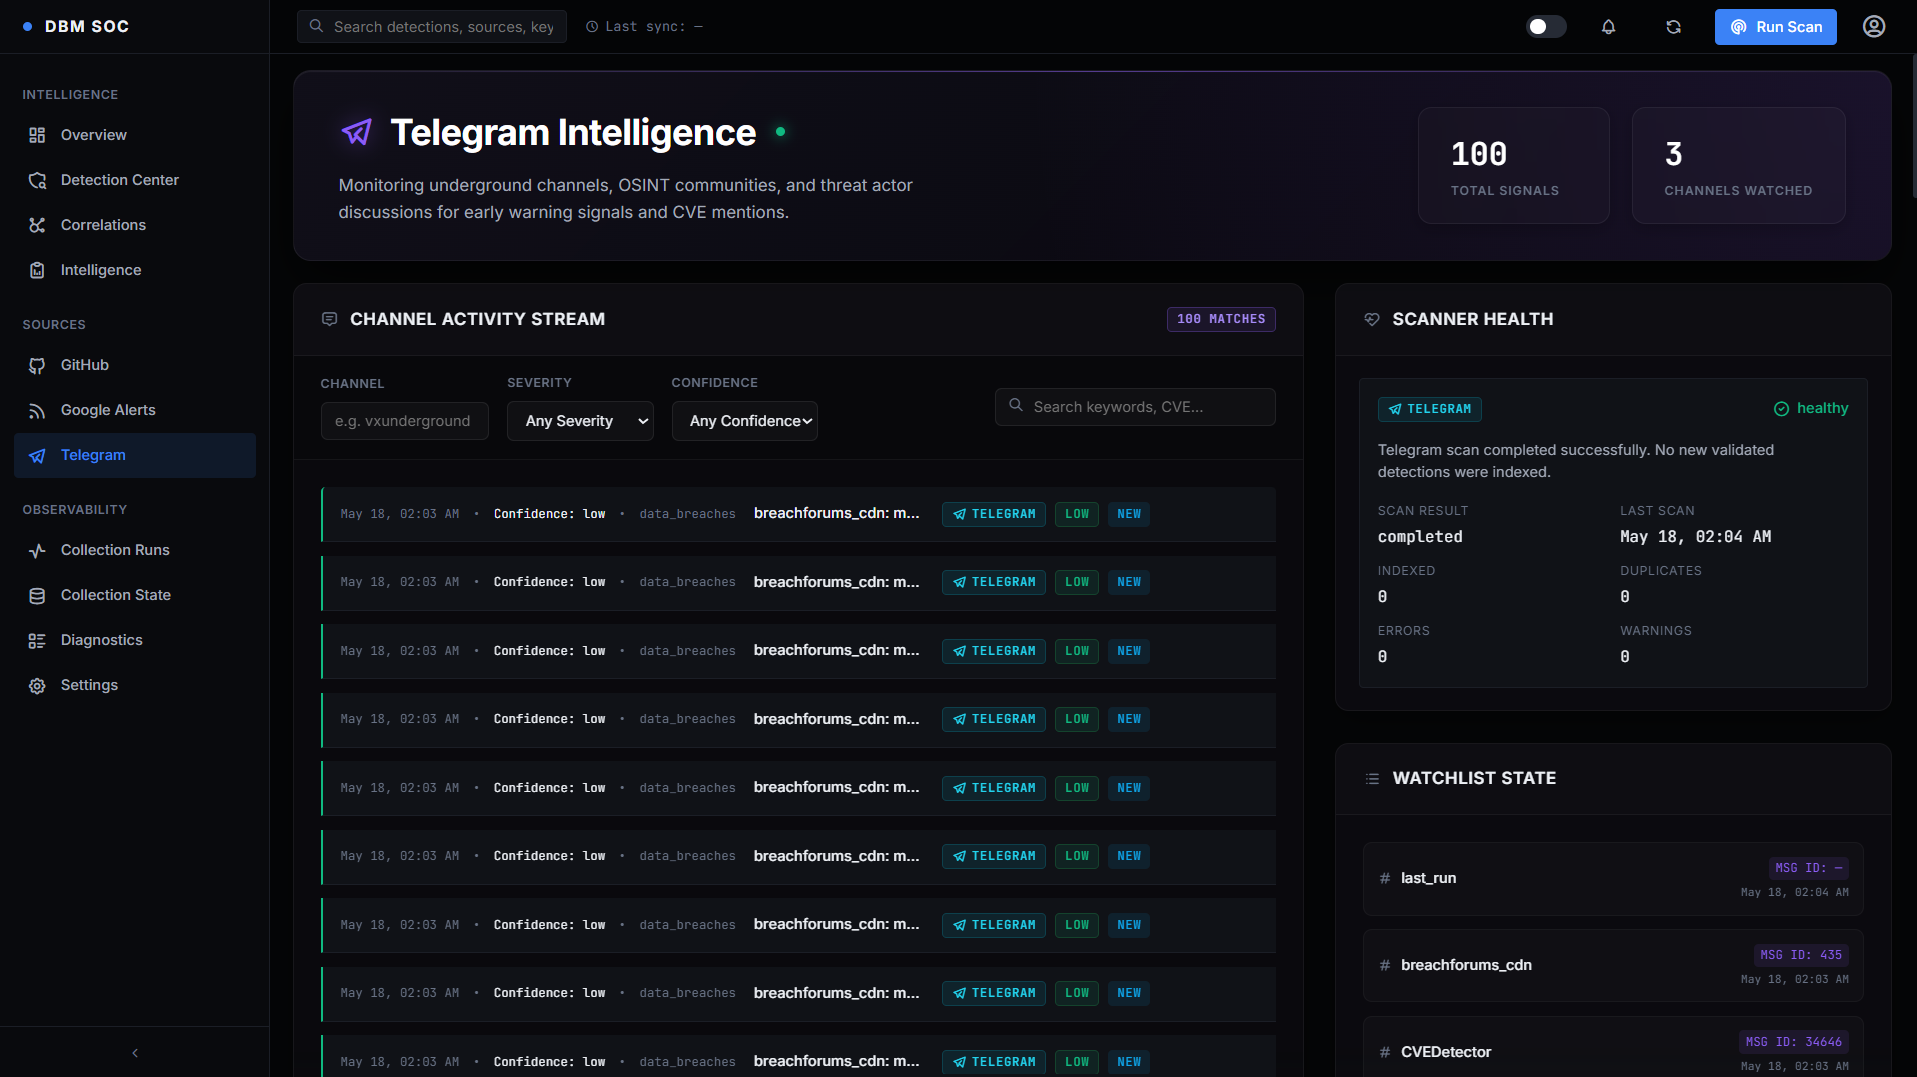
\includegraphics[width=.9\linewidth]{images/tg_dash.png}
    \caption{Interface Telegram Monitoring affichant les signaux collectés depuis les canaux publics}
    \label{fig:telegram-dashboard}
\end{figure}

\subsection{Exemple de signal Telegram}

Un exemple de signal collecté depuis le canal \texttt{breachforums\_cdn} concerne une annonce publique mentionnant une fuite liée à \textbf{Avito.ma}. Le message indique qu'environ \textbf{2,7 millions d'enregistrements} auraient été exposés à la suite d'un incident datant approximativement de septembre 2022.

\begin{itemize}
  \item source du signal : canal Telegram public \texttt{breachforums\_cdn} ;
  \item organisation mentionnée : \textbf{Avito.ma} ;
  \item volume annoncé : environ \textbf{2,728,091 enregistrements} ;
  \item type de signal : annonce de fuite de données ;
  \item statut analytique : information à valider par corrélation avec d'autres sources.
\end{itemize}

Ce type de message ne constitue pas automatiquement une preuve technique. Il représente plutôt un signal OSINT qui doit être enrichi, vérifié et comparé avec d'autres sources avant d'être considéré comme un incident confirmé.

\begin{figure}[H]
    \centering
    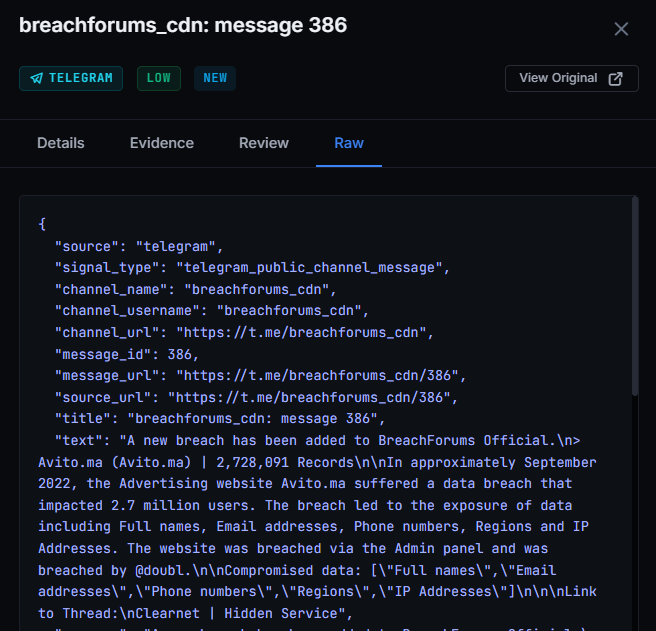
\includegraphics[width=.8\linewidth]{images/tg_exposure.png}
    \caption{Exemple de signal Telegram lié à une annonce publique de fuite de données}
    \label{fig:telegram-exposure}
\end{figure}

\newpage
\section{Google Alerts Monitoring}

\subsection{Rôle de la source}

Google Alerts apporte la dimension \textbf{news / OSINT} au pipeline de veille. Cette source permet de capter, à grande échelle et en quasi-temps réel, la couverture médiatique des incidents de sécurité, des fuites de données et des compromissions d'entreprises.

\subsection{Configuration des alertes}

Au total, \textbf{16 alertes personnalisables} ont été configurées. Chaque alerte est définie par :

\begin{itemize}
  \item un nom ;
  \item une catégorie ;
  \item un pays ou périmètre géographique ;
  \item une requête ciblée en français et en anglais ;
  \item une URL RSS produite par Google Alerts.
\end{itemize}

\begin{table}[H]
\centering
\caption{Exemples de catégories d'alertes configurées}
\label{tab:alerts-categories}
\begin{tabularx}{\linewidth}{|l|>{\raggedright\arraybackslash}X|}
\hline
\rowcolor{primary!15}
\textbf{Catégorie} & \textbf{Sujet surveillé} \\ \hline
global\_cyber\_incidents & Cyberattaques et fuites à grande échelle \\ \hline
ransomware\_monitoring & Incidents et groupes ransomware \\ \hline
healthcare\_breaches & Hôpitaux et données médicales \\ \hline
financial\_incidents & Banques, fintech, fraudes \\ \hline
government\_incidents & Secteur public et contractants défense \\ \hline
zero\_day\_vulnerabilities & 0-day et CVE activement exploités \\ \hline
dark\_web\_activity & Ventes de données, brokers d'accès \\ \hline
anssi\_cert\_fr & Bulletins officiels ANSSI / CERT-FR \\ \hline
\end{tabularx}
\end{table}


\begin{figure}[H]
    \centering
    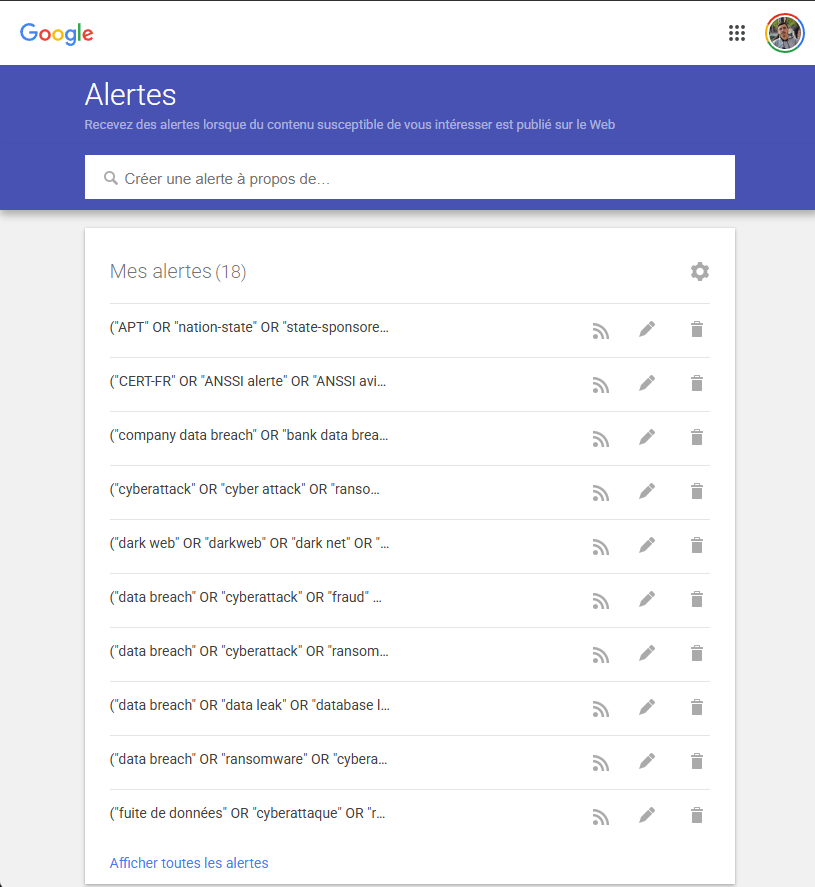
\includegraphics[width=.85\linewidth]{images/gaw.png}
    \caption{image sur l(interface google alerts}
\end{figure}


\subsection{Logique d'exploitation}

Les flux RSS sont récupérés à intervalle régulier. Pour chaque entrée, la plateforme extrait les métadonnées, rattache la détection à sa catégorie d'origine, applique des règles de filtrage et conserve uniquement l'information normalisée et redactée.

\begin{figure}[H]
    \centering
    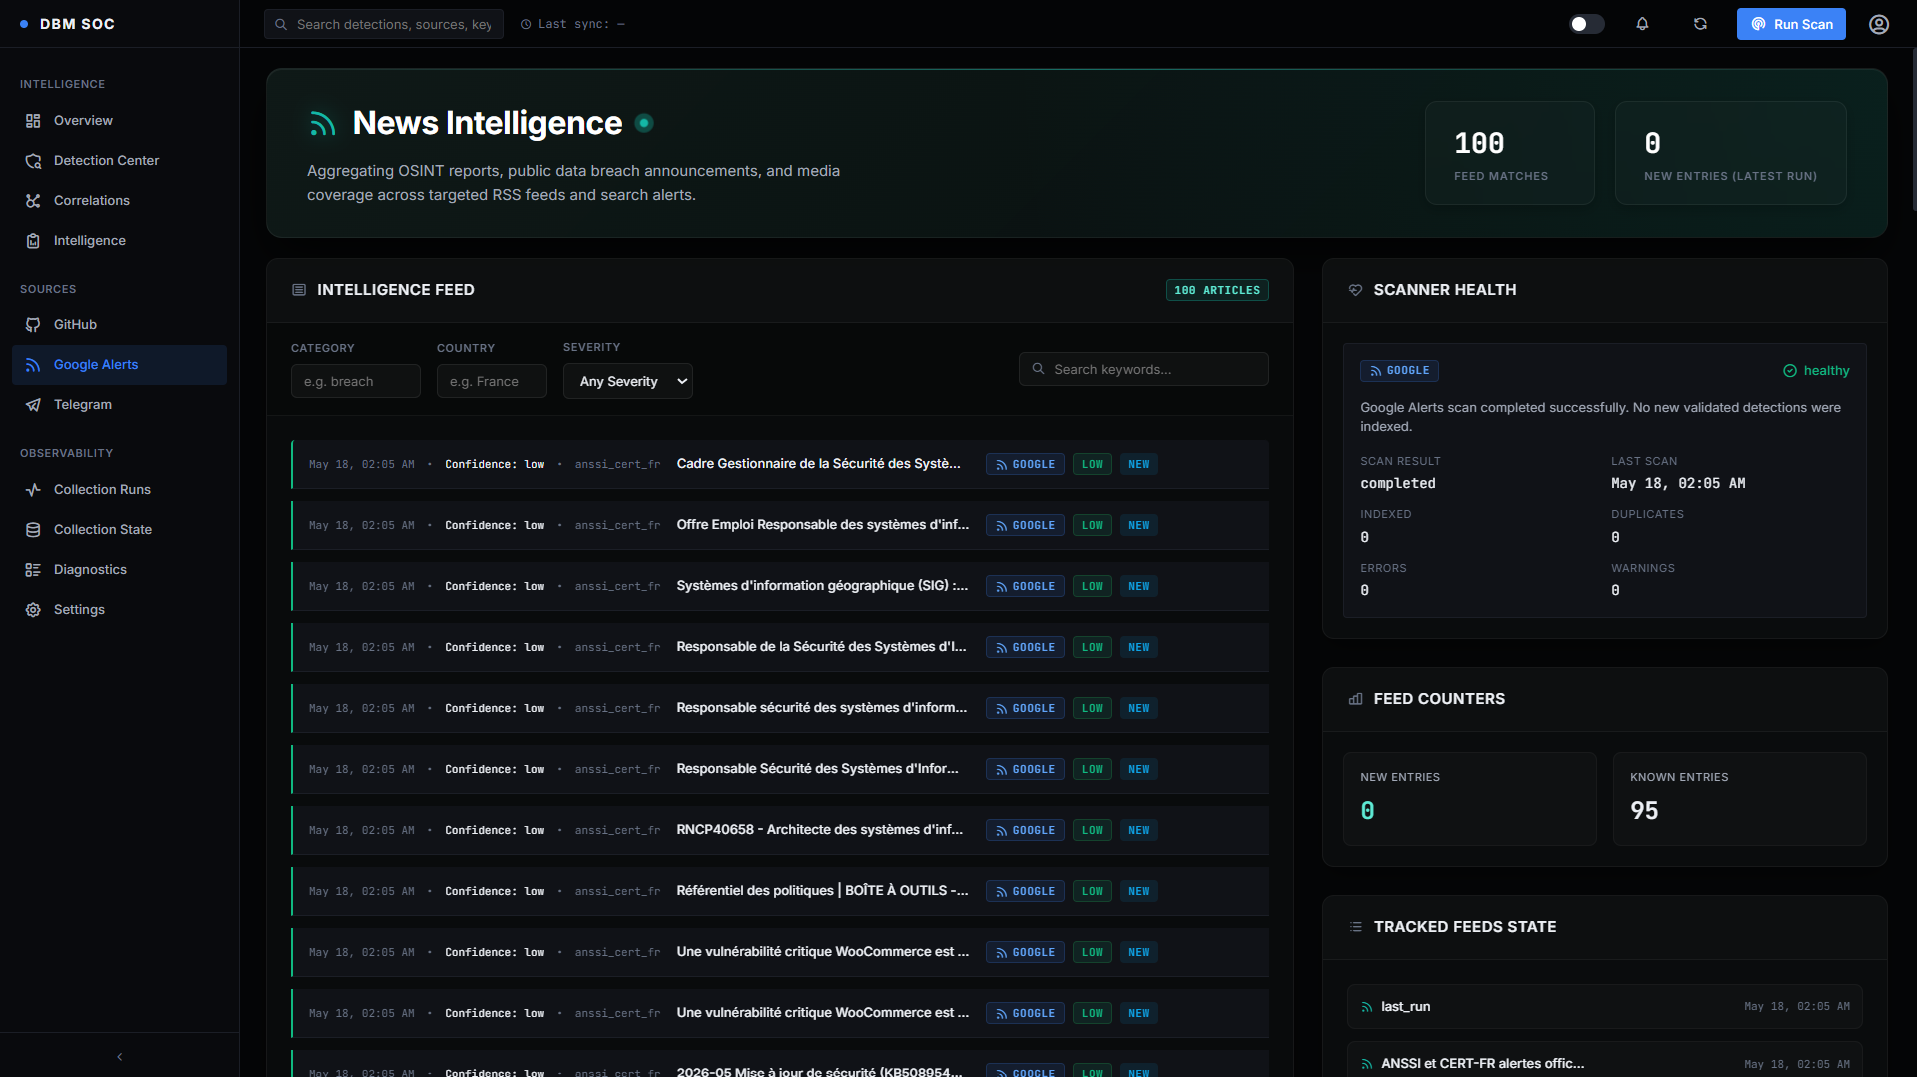
\includegraphics[width=1\linewidth]{images/ga.png}
    \caption{Interface de suivi des alertes Google Alerts}
    \label{fig:google-alerts}
\end{figure}

\section{CVE Feed et BI Threat Intelligence}

\subsection{Positionnement du module}

Le module \textit{BI Threat Intelligence} est un projet complémentaire à la plateforme \projetnom{}. Contrairement aux modules GitHub, Telegram ou Google Alerts, qui se concentrent sur la détection d'expositions et de signaux cyber, ce module est orienté vers l'exploitation analytique des flux \textbf{Common Vulnerabilities and Exposures}.

Son objectif principal est de collecter, structurer et analyser les données CVE afin de produire une vision décisionnelle sur l'évolution des vulnérabilités dans le temps.

\subsection{Architecture du pipeline CVE}

Le module repose sur une architecture de type \textbf{Data Warehouse} organisée selon le modèle médaillon.

\begin{itemize}
  \item \textbf{Bronze Layer} : ingestion brute des données CVE depuis les sources externes ;
  \item \textbf{Silver Layer} : nettoyage, normalisation, enrichissement et déduplication ;
  \item \textbf{Gold Layer} : création des agrégats métiers, indicateurs de risque et tables prêtes pour Power BI.
\end{itemize}

\begin{figure}[H]
    \centering
    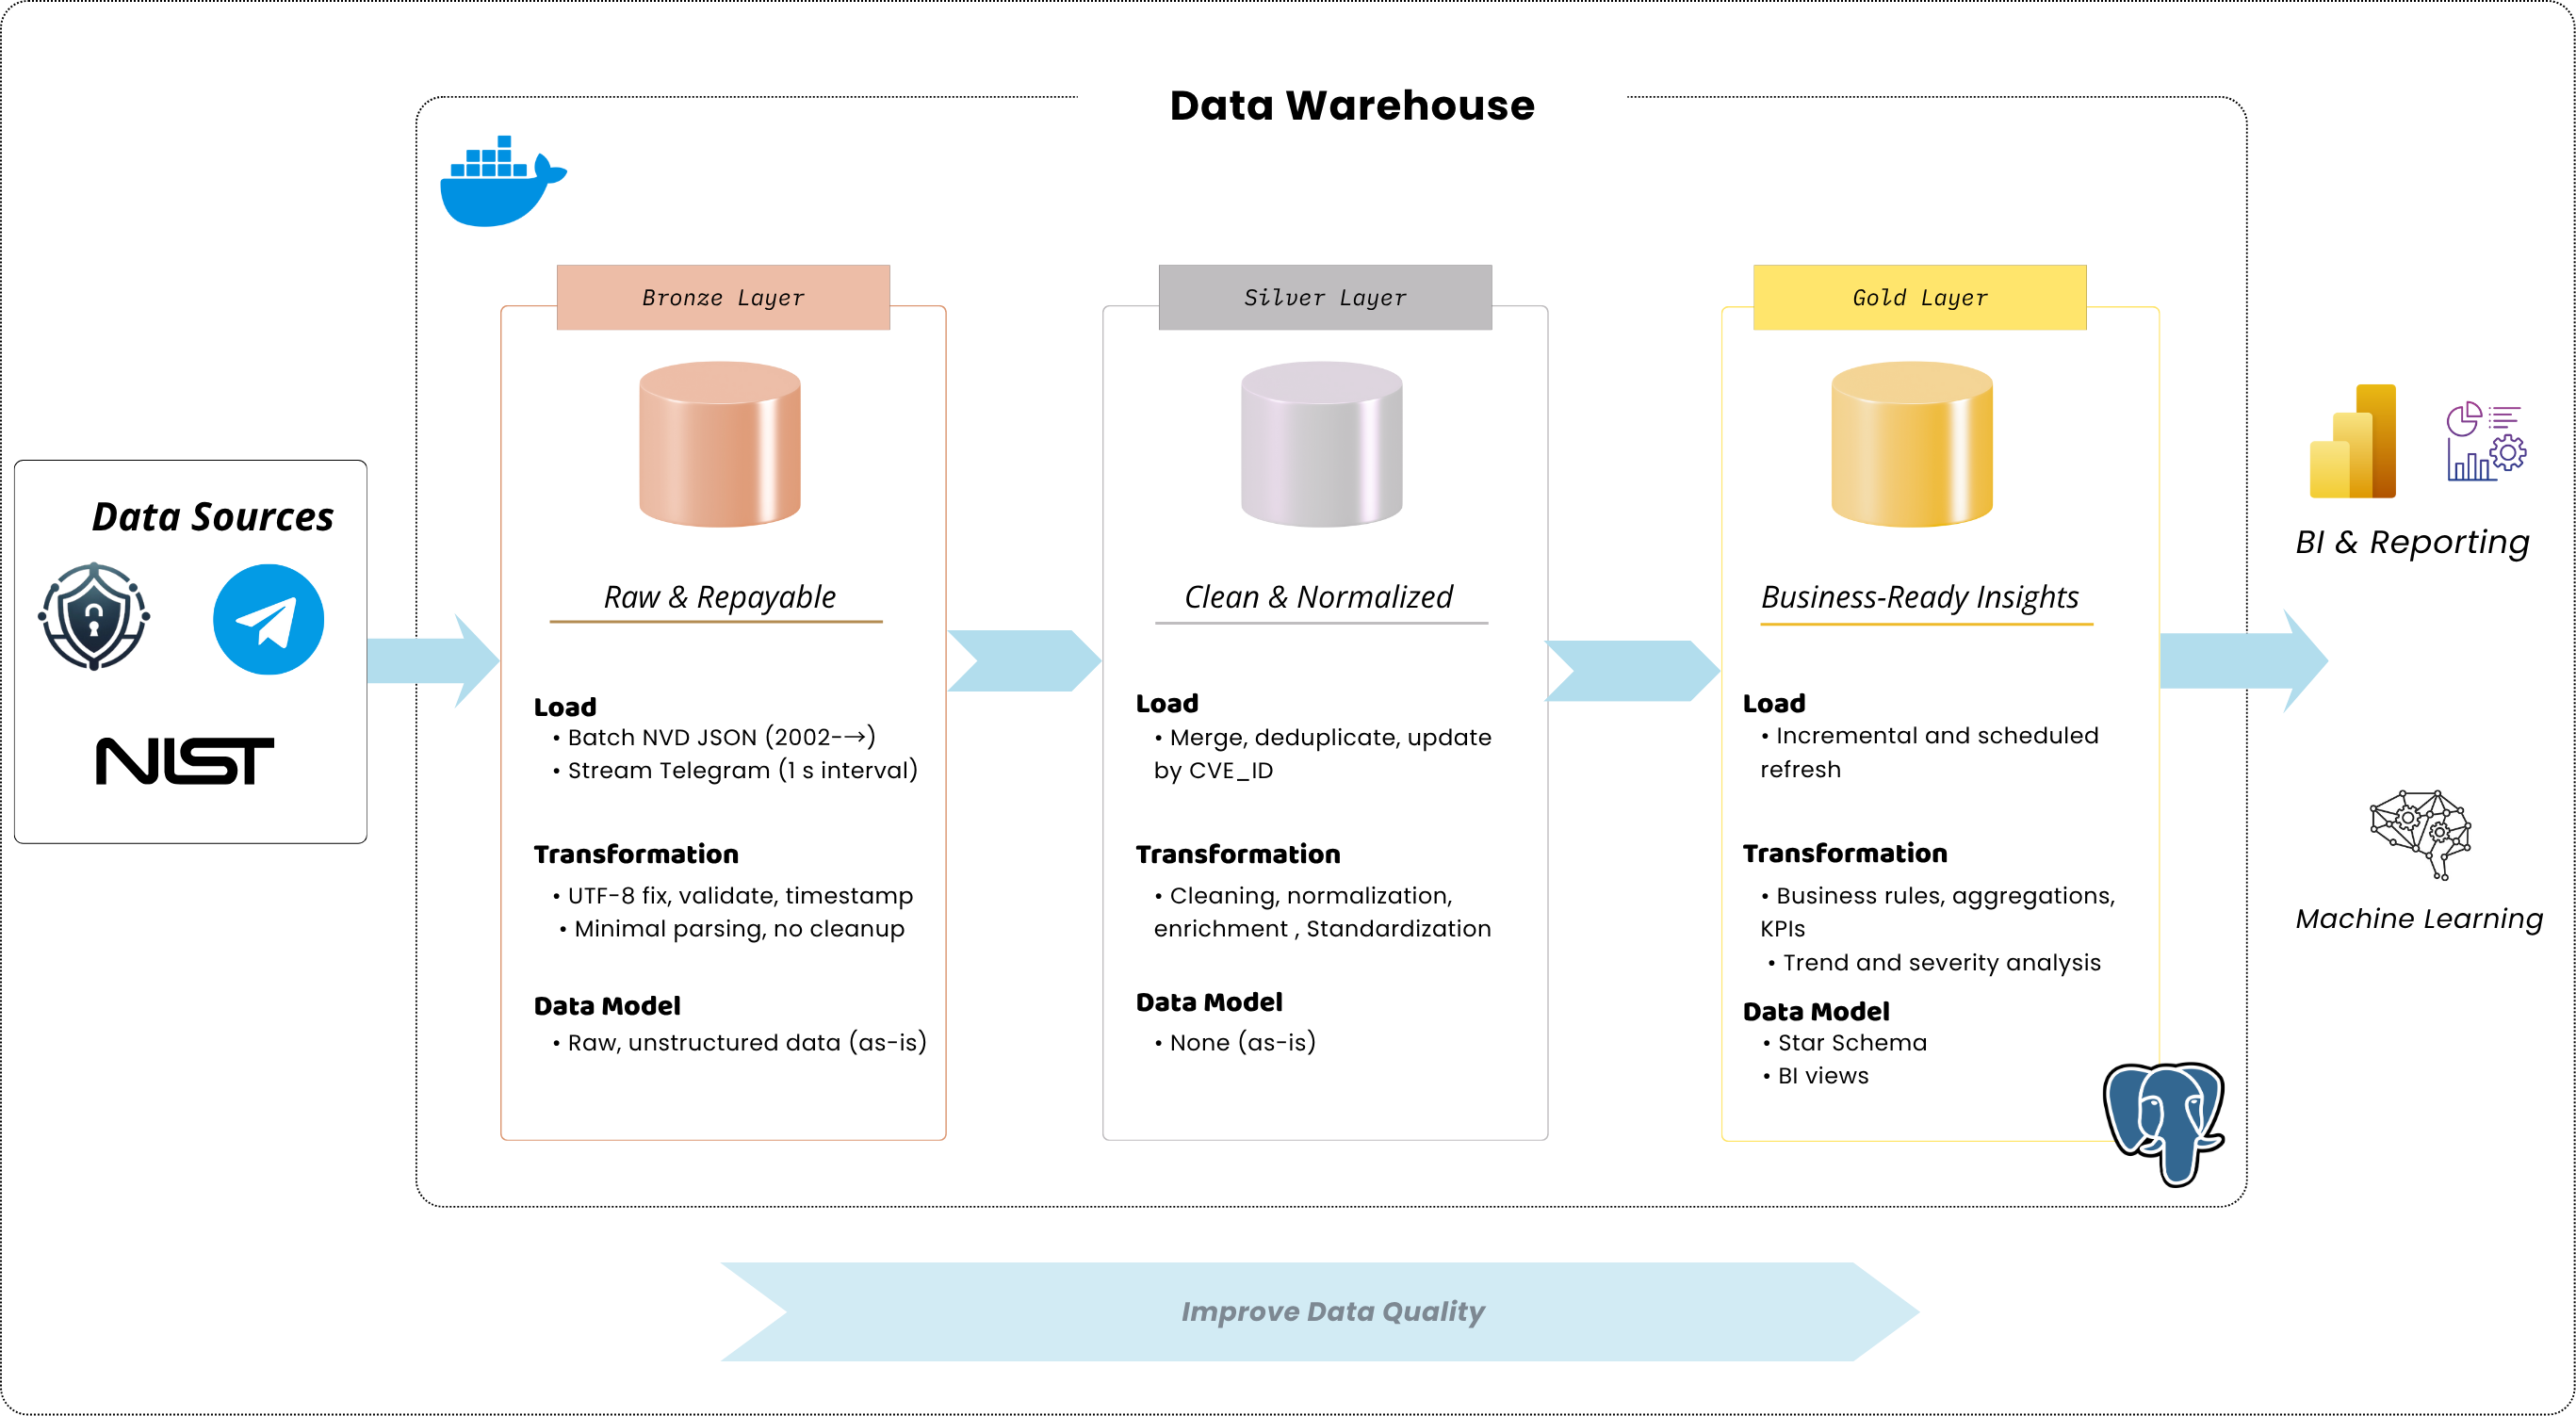
\includegraphics[width=1\linewidth]{images/TIP.png}
    \caption{Architecture du pipeline BI Threat Intelligence basée sur les couches Bronze, Silver et Gold}
    \label{fig:tip-architecture}
\end{figure}



\section{Rôle des tableaux de bord}

La restitution constitue la dernière étape du pipeline. Elle transforme les signaux qualifiés en informations exploitables par l'analyste. Les tableaux de bord permettent de suivre les résultats collectés, l'état des sources, les erreurs, les avertissements, les tendances et les exemples de détections.

L'objectif n'est pas seulement d'afficher des données, mais de fournir une interface de revue permettant d'identifier rapidement les signaux importants.

\section{Tableaux de bord Power BI}

Le module \textit{BI Threat Intelligence} fournit trois pages principales dans le dashboard Power BI. Chaque page répond à un objectif analytique différent.

\subsection{Executive Overview}

La page \textbf{Executive Overview} donne une vision globale de l'état des vulnérabilités. Elle présente les principaux indicateurs, notamment le nombre total de CVE, le volume de vulnérabilités critiques, les fournisseurs impactés et le pourcentage de CVE critiques.

Elle permet également de visualiser l'évolution annuelle des CVE, les fournisseurs les plus concernés et la répartition des vulnérabilités par niveau de sévérité.

\begin{figure}[H]
    \centering
    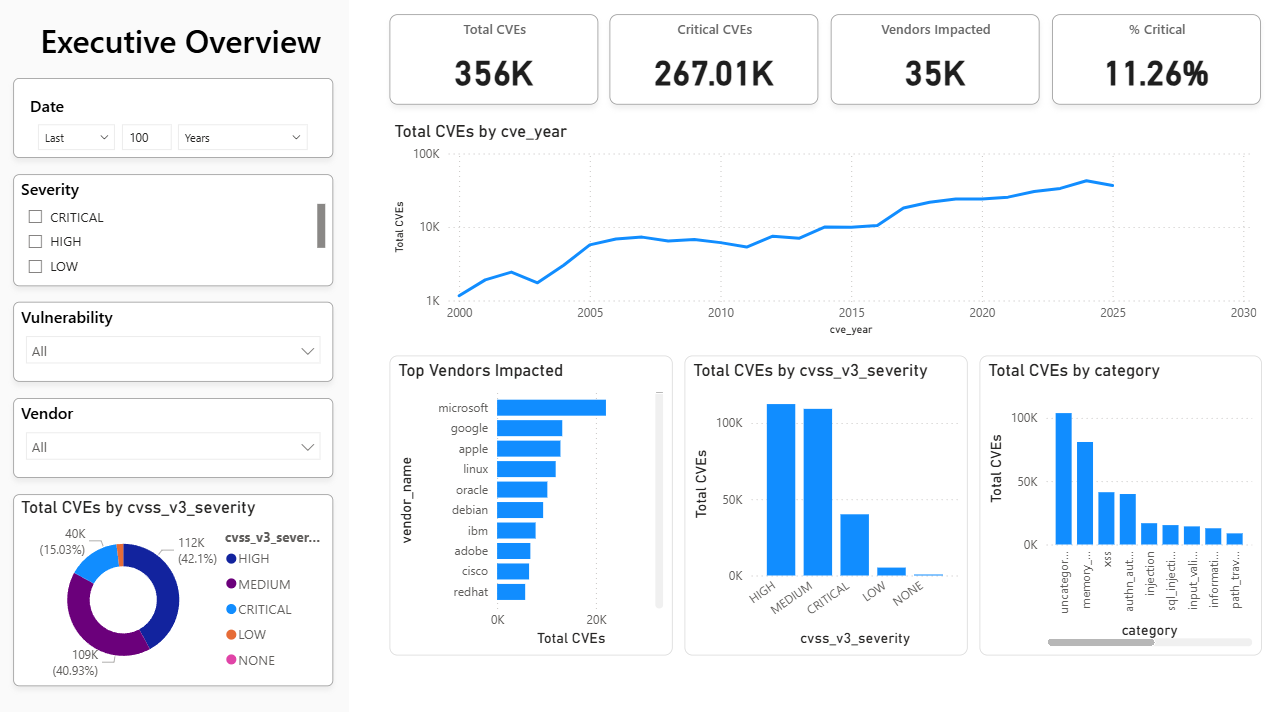
\includegraphics[width=1\linewidth]{images/Executive Overview.png}
    \caption{Dashboard Power BI -- Executive Overview des vulnérabilités CVE}
    \label{fig:executive-overview}
\end{figure}

\subsection{Time and Age Analysis}

La page \textbf{Time and Age Analysis} analyse les CVE selon leur dimension temporelle. Elle permet d'observer l'évolution du nombre de vulnérabilités par année, les tendances mensuelles, ainsi que la distribution des CVE selon leur ancienneté.

Cette page aide à comprendre si les vulnérabilités sont principalement récentes ou anciennes, et comment les niveaux de sévérité se répartissent selon l'âge des CVE.

\begin{figure}[H]
    \centering
    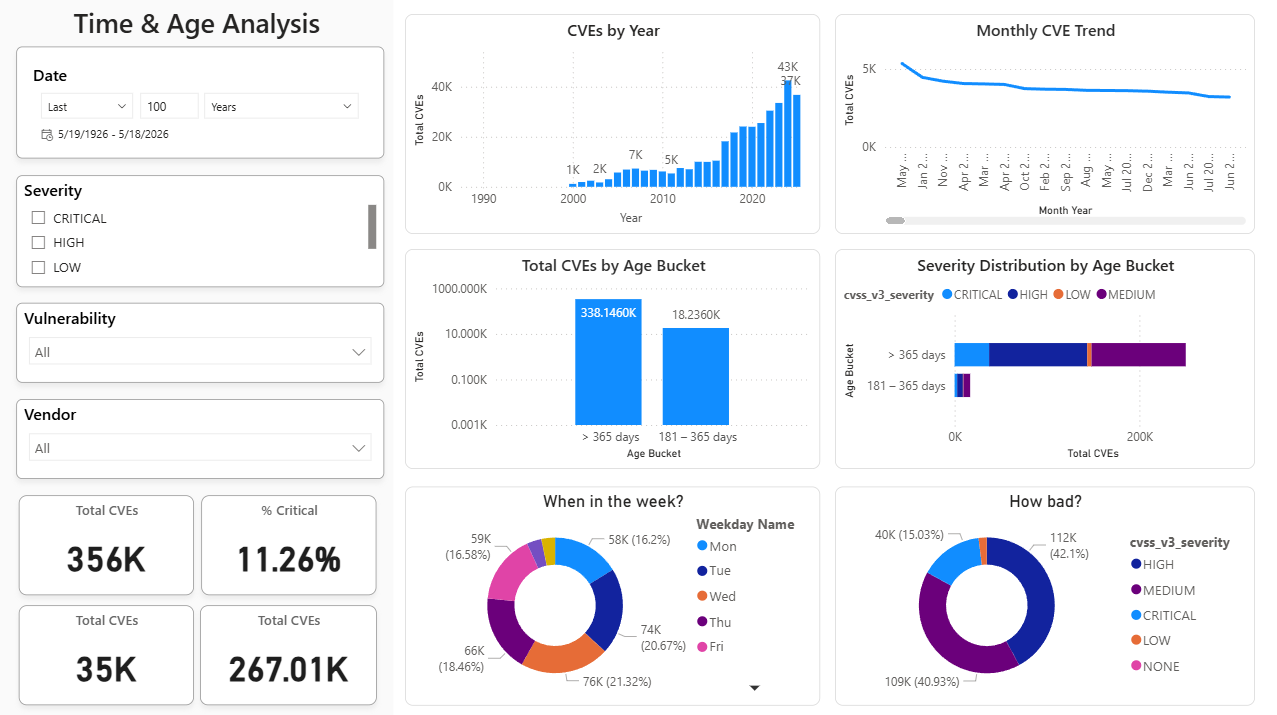
\includegraphics[width=1\linewidth]{images/Time & Age Analysis.png}
    \caption{Dashboard Power BI -- Analyse temporelle et ancienneté des CVE}
    \label{fig:time-age-analysis}
\end{figure}

\subsection{Severity and Impact Analysis}

La page \textbf{Severity and Impact Analysis} se concentre sur l'analyse de la criticité et de l'impact des vulnérabilités. Elle présente la distribution des sévérités, les scores CVSS moyens et maximums, ainsi que la relation entre impact et exploitabilité.

Cette page permet d'identifier les vulnérabilités les plus critiques et d'avoir une lecture plus fine du risque à travers les métriques CVSS.

\begin{figure}[H]
    \centering
    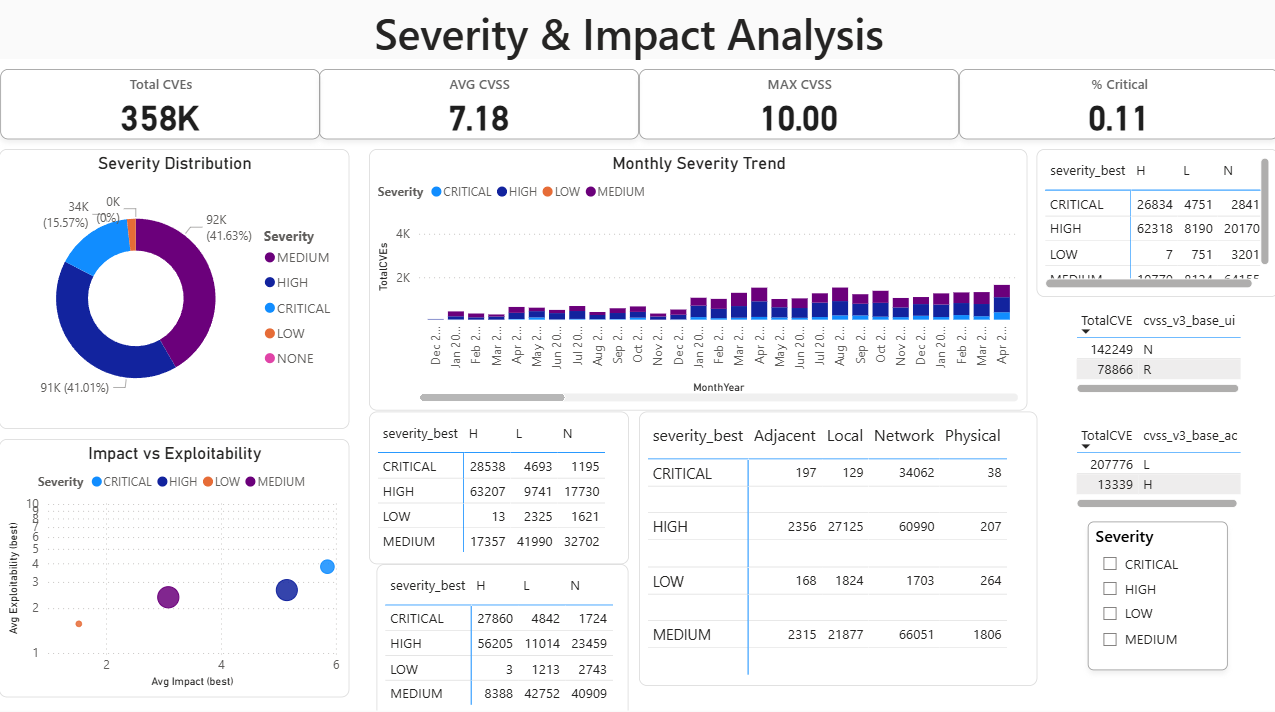
\includegraphics[width=1\linewidth]{images/Severity & Impact Analysis.png}
    \caption{Dashboard Power BI -- Analyse de la sévérité et de l'impact des CVE}
    \label{fig:severity-impact-analysis}
\end{figure}

\section{Apport analytique du module BI}

Le module CVE Feed et BI Threat Intelligence transforme les flux CVE en indicateurs décisionnels. Il permet à l'analyste de comprendre l'évolution des vulnérabilités, d'identifier les tendances importantes et de mieux prioriser les risques.

Cette brique apporte une dimension analytique au projet global. Elle ne détecte pas seulement des signaux cyber, mais fournit une vision historique, statistique et stratégique de l'écosystème des vulnérabilités.

\section{Synthèse des résultats obtenus}

Le projet permet de centraliser plusieurs types de signaux cyber dans un même environnement. GitHub apporte les preuves techniques d'exposition, Telegram fournit des signaux communautaires précoces, Google Alerts ajoute une couverture médiatique OSINT, et le module CVE offre une lecture quantitative des vulnérabilités.

La combinaison de ces sources permet de construire une démarche de veille plus complète, dans laquelle chaque signal peut être collecté, qualifié, visualisé et exploité par un analyste.


% =============================================================================
%  CHAPITRE 4 — TRAITEMENT, DÉTECTION ET CLASSIFICATION DES RISQUES
% =============================================================================
\chapter{Traitement, détection et classification des risques}

\section{Méthodologie de collecte}

La collecte s'opère selon deux régimes complémentaires.

\begin{itemize}
  \item \textbf{Collecte planifiée} : un planificateur exécute périodiquement les collecteurs afin d'assurer une couverture continue.
  \item \textbf{Collecte à la demande} : l'analyste peut déclencher un scan immédiat depuis l'interface pour valider un changement de configuration ou enquêter sur un signal.
\end{itemize}

\section{Limites de volumétrie}

Pour préserver la stabilité du service et respecter les quotas externes, chaque source applique des plafonds de volumétrie configurables : nombre maximal de requêtes par exécution, nombre maximal d'éléments par requête, nombre maximal de récupérations de contenu et taille maximale du contenu téléchargé.

Cette discipline est essentielle pour transformer une collecte ponctuelle en une chaîne de veille soutenable dans la durée.

\section{Déduplication}

Toute détection est associée à un \textbf{hash de déduplication}. Lorsqu'un nouveau passage de collecte rapporte une donnée déjà connue, la plateforme l'ignore avant l'indexation.

Ce mécanisme évite la pollution de la base de détections et explique pourquoi le total indexé peut rester stable malgré une activité de collecte réelle.

\section{Vue d'ensemble des passages de collecte}

Chaque exécution est enregistrée dans une trace dédiée appelée \textit{collection run}. Cette trace détaille la source concernée, la date du passage, sa durée, le nombre d'éléments collectés, indexés, dédupliqués, ainsi que les erreurs et avertissements éventuels.
\begin{figure}[H]
    \centering
    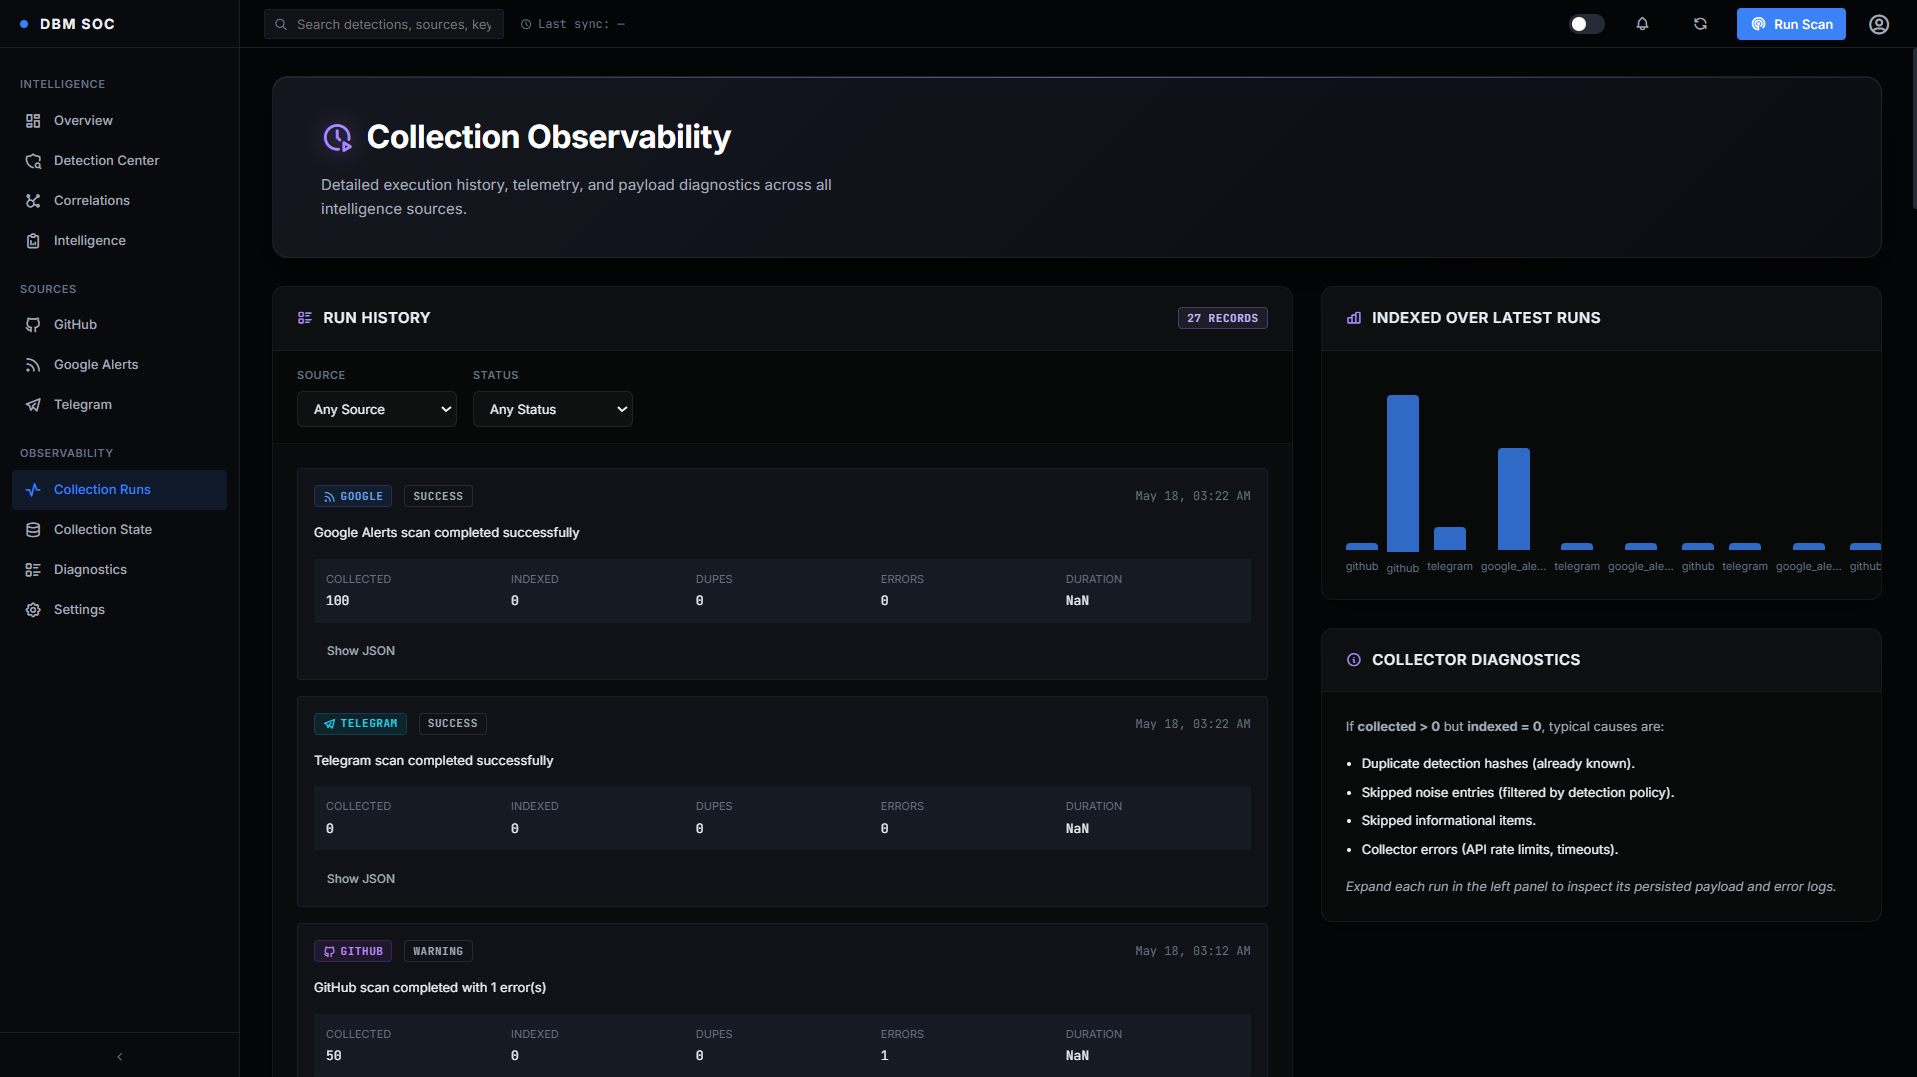
\includegraphics[width=.9\linewidth]{images/collection.png}
\end{figure}

\section{Normalisation des données}

Les sources ne produisent pas le même type de données : GitHub retourne du code, Telegram du texte de message, Google Alerts des entrées RSS et les flux CVE des objets structurés. Une étape de normalisation est donc nécessaire.

Cette étape transforme chaque résultat brut en un document de détection unifié comportant des champs communs : source, URL publique, titre, organisation éventuellement concernée, catégorie de risque, indicateurs détectés, texte redacté, score, sévérité, statut analyste et horodatages.

\section{Analyse du contenu}

L'analyse de contenu vise à extraire les indicateurs qui donnent de la valeur à une détection. Selon la source, il peut s'agir :

\begin{itemize}
  \item de motifs de secrets dans du code ;
  \item de mentions explicites de fuites de données ;
  \item de mentions d'organisations victimes ;
  \item de références CVE ;
  \item de métadonnées liées à la source ou à la catégorie d'alerte.
\end{itemize}

\section{Filtrage}

Le filtrage applique plusieurs catégories de règles complémentaires.

\begin{itemize}
  \item \textbf{Filtres de valeurs placeholders} : élimination des chaînes comme \textit{changeme}, \textit{your\_key}, \textit{example} ou \textit{xxx}.
  \item \textbf{Filtres d'emplacement} : exclusion des dossiers et fichiers manifestement d'exemple comme \texttt{tests/}, \texttt{docs/}, \texttt{examples/} ou \texttt{.env.example}.
  \item \textbf{Filtres de score} : exigence d'un score minimum pour qu'une détection puisse être indexée.
\end{itemize}

\section{Detection policy}

La \textit{detection policy} est le garde-fou central de la plateforme. Elle décide si une donnée brute mérite d'être conservée et détermine sa sévérité.

Elle permet notamment de :

\begin{itemize}
  \item vérifier le contenu réel du fichier et non uniquement son nom ;
  \item identifier les secrets potentiellement exploitables ;
  \item exclure les faux positifs fréquents ;
  \item réduire la confiance des chemins d'exemple ;
  \item calculer un score de risque ;
  \item associer une sévérité au signal ;
  \item masquer les valeurs sensibles avant stockage.
\end{itemize}


\section{Classification des risques}

Chaque détection retenue est classée selon plusieurs axes.

\begin{enumerate}
  \item \textbf{Catégorie de risque} : \texttt{env\_files}, \texttt{database\_credentials}, \texttt{api\_keys}, \texttt{cloud\_keys}, \texttt{jwt\_tokens}, \texttt{private\_keys}, \texttt{docker\_secrets}, etc.
  \item \textbf{Niveau de criticité} : \textit{low}, \textit{medium}, \textit{high}.
  \item \textbf{Niveau de confiance} : \textit{low}, \textit{medium}, \textit{high}.
  \item \textbf{Statut analyste} : \textit{new}, \textit{reviewed}, \textit{false\_positive}, \textit{confirmed}, \textit{escalated}.
\end{enumerate}

\begin{table}[H]
\centering
\caption{Axes de classification des détections}
\label{tab:classification}
\begin{tabularx}{\linewidth}{|l|>{\raggedright\arraybackslash}X|}
\hline
\rowcolor{primary!15}
\textbf{Axe} & \textbf{Valeurs possibles} \\ \hline
Source & github, telegram, google\_alerts, mock\_paste \\ \hline
Catégorie de risque & env\_files, database\_credentials, api\_keys, cloud\_keys, jwt\_tokens, private\_keys, docker\_secrets, framework\_configs \\ \hline
Sévérité & low, medium, high \\ \hline
Confiance & low, medium, high \\ \hline
Statut analyste & new, reviewed, ignored, confirmed, false\_positive, escalated \\ \hline
\end{tabularx}
\end{table}

\section{Gestion des faux positifs}

La plateforme ne considère pas automatiquement chaque résultat brut comme un incident. Certains contenus peuvent ressembler à des secrets sans être réellement exploitables. C'est le cas des fichiers d'exemple, des valeurs placeholders ou des contenus volontairement fictifs.

La détection initiale reste utile, car elle identifie un candidat. Cependant, l'analyse de contenu et la \textit{detection policy} permettent de distinguer un vrai secret exploitable d'un contenu de test ou d'un faux positif.




% =============================================================================
%  CONCLUSION GÉNÉRALE
% =============================================================================
\chapter*{Conclusion générale}
\addcontentsline{toc}{chapter}{Conclusion générale}

Le projet \textit{\projetnom{}} a permis de concevoir et de mettre en œuvre une plateforme de veille cyber cohérente, qui traite la veille comme un processus méthodologique et non comme une simple accumulation de logs.

À travers quatre sources complémentaires --- GitHub pour les preuves techniques, Telegram pour le signal communautaire, Google Alerts pour la dimension médiatique, et le module BI Threat Intelligence pour les vulnérabilités CVE --- la plateforme couvre un large spectre d'expositions publiques et de signaux cyber.

La méthodologie repose sur une séparation claire entre la collecte, l'analyse, la classification et la restitution. Cette séparation donne au système une meilleure lisibilité, une meilleure maintenabilité et une capacité d'évolution plus importante.

Au-delà de l'apport technique, ce projet constitue un exercice méthodologique. Il montre comment, en s'appuyant sur des sources ouvertes et autorisées, il est possible de construire une chaîne de veille rigoureuse, défensive et exploitable, en cohérence avec les exigences académiques d'un projet de fin d'études.

Les perspectives identifiées, comme l'amélioration de la corrélation, l'automatisation des rapports et l'enrichissement des indicateurs, ouvrent la voie à un passage progressif d'un outil pédagogique vers un véritable outil opérationnel. 

% =============================================================================
\end{document} 